\chapter{Projeto e Implementação da Solução}
\label{chapter:solução}

\section{Introdução}

Este capítulo apresenta o processo de desenvolvimento da solução proposta, desde a construção física da mão robótica até à implementação do sistema sensorial.  Inicia-se com a apresentação das etapas associadas ao fabrico e montagem da estrutura da mão robótica, seguindo-se a configuração dos motores e o desenvolvimento da lógica de controlo, desde o acionamento de motores individuais até ao controlo coordenado da mão completa.

É igualmente descrita a arquitetura de software desenvolvida, com especial destaque para as funcionalidades avançadas implementadas, como o ajuste dinâmico de corrente durante o contacto com objetos, a definição de velocidades relativas entre dedos e falanges, e a introdução de atrasos temporais entre movimentos.

Adicionalmente, aborda-se a implementação do sistema sensorial de deteção de contacto, incluindo a seleção do microcontrolador, o desenvolvimento físico da unidade de aquisição e os testes realizados com diferentes sensores. 

\section{Desenvolvimento da Mão Robótica}



\subsection{Fabrico e Montagem da estrutura}

A construção da estrutura da mão robótica seguiu integralmente as indicações fornecidas na documentação da LEAP Hand, a qual disponibiliza de forma aberta e acessível todos os ficheiros CAD necessários, bem como instruções detalhadas de montagem. Esta abordagem permitiu realizar uma primeira montagem da estrutura de forma fiel ao projeto original, facilitando a replicação inicial da arquitetura mecânica.

As peças foram produzidas por impressão 3D com recurso a uma Creality K1, uma impressora de alto desempenho que assegura uma boa qualidade dimensional e tempos de fabrico reduzidos. Para a estrutura principal foi utilizado o filamento Hyper PLA da Creality, selecionado pela sua rigidez e facilidade de impressão. Já para as pontas dos dedos, onde se pretende maior flexibilidade e capacidade de aderência ao contacto com objetos, foi utilizado o Python Flex TPU da FormFutura.

A construção dos dedos revelou-se a fase mais demorada do processo de montagem, devido ao elevado número de componentes envolvidos e à complexidade dos passos necessários. Todos os dedos seguem a mesma configuração estrutural, com exceção do polegar, que apresenta um desenho distinto adaptado à sua função anatómica e posição na mão.

Na Figura~\ref{fig:polegar} é apresentado o polegar já montado, enquanto na Figura~\ref{fig:dedo} observa-se um dos restantes dedos, com estrutura idêntica entre si. A montagem de cada dedo envolveu operações detalhadas e sequenciais que exigiram precisão e atenção redobrada, especialmente na organização dos cabos e no alinhamento das juntas móveis.

\begin{figure}[H]
    \centering
    \begin{minipage}[b]{0.45\textwidth}
        \centering
        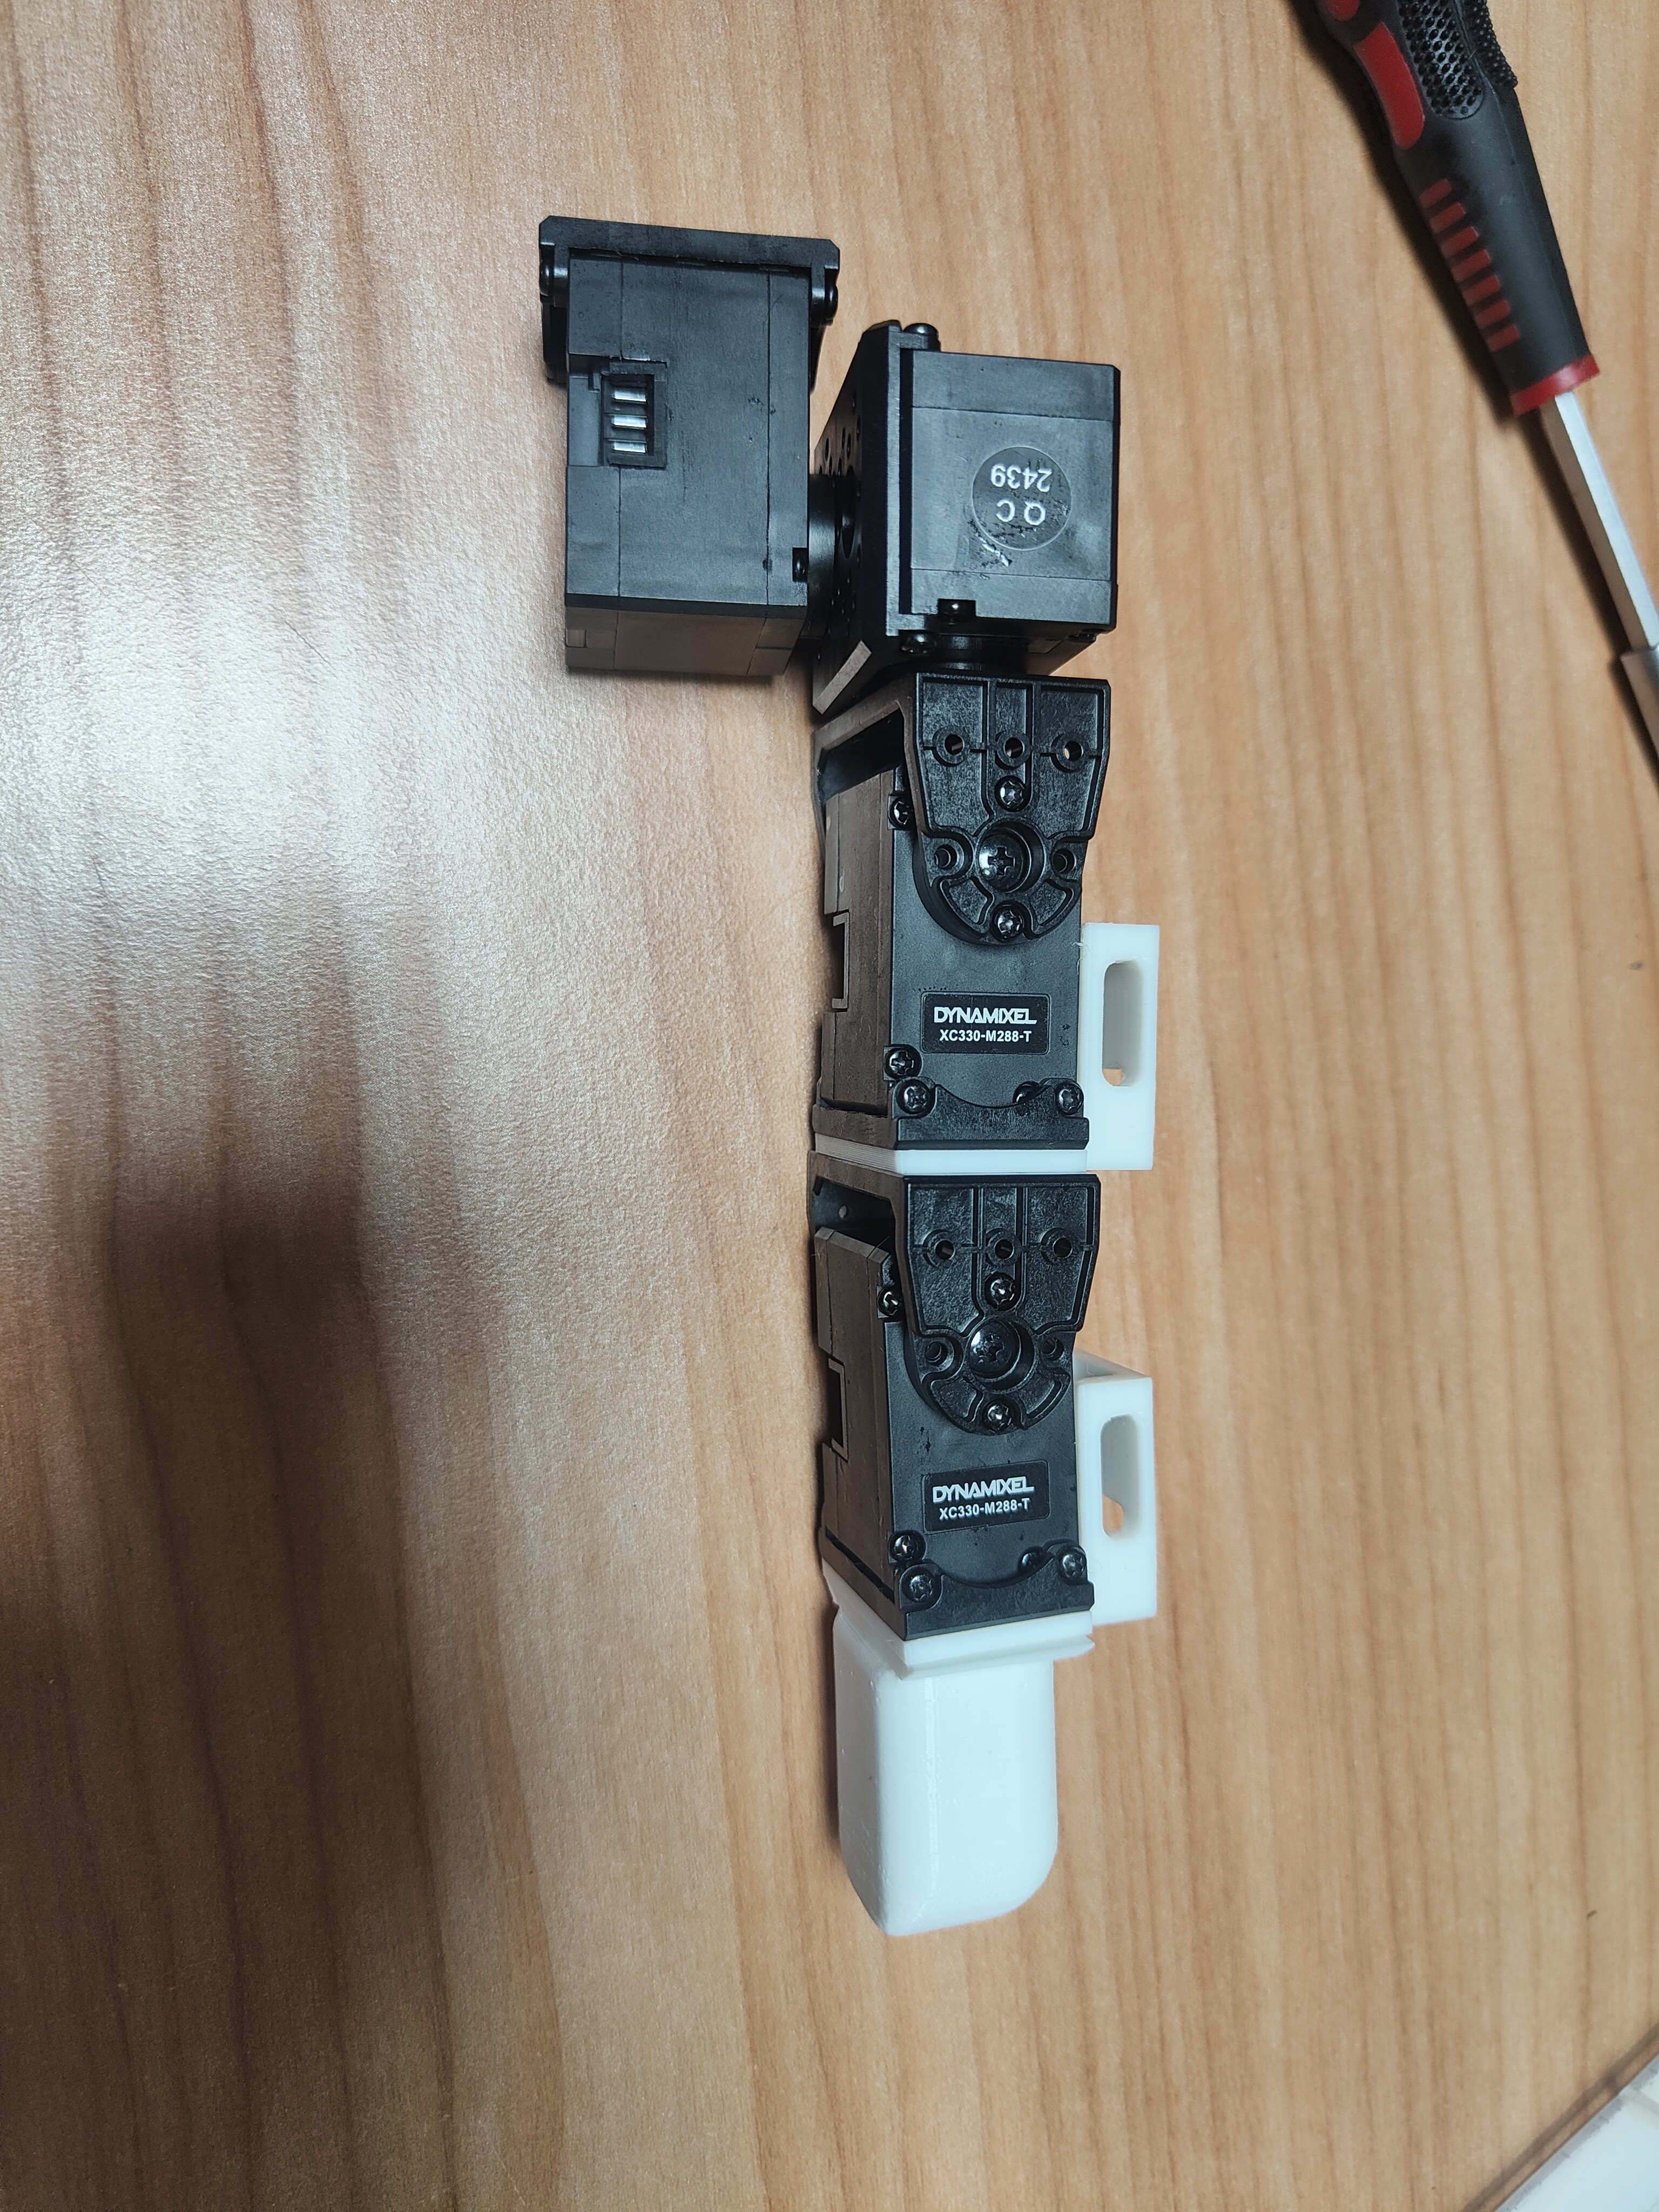
\includegraphics[height=6cm]{figs/chapter4/polegar.jpg}
        \caption{Polegar construído de acordo com a Documentação da Leap Hand}
        \label{fig:polegar}
    \end{minipage}
    \hfill
    \begin{minipage}[b]{0.45\textwidth}
        \centering
        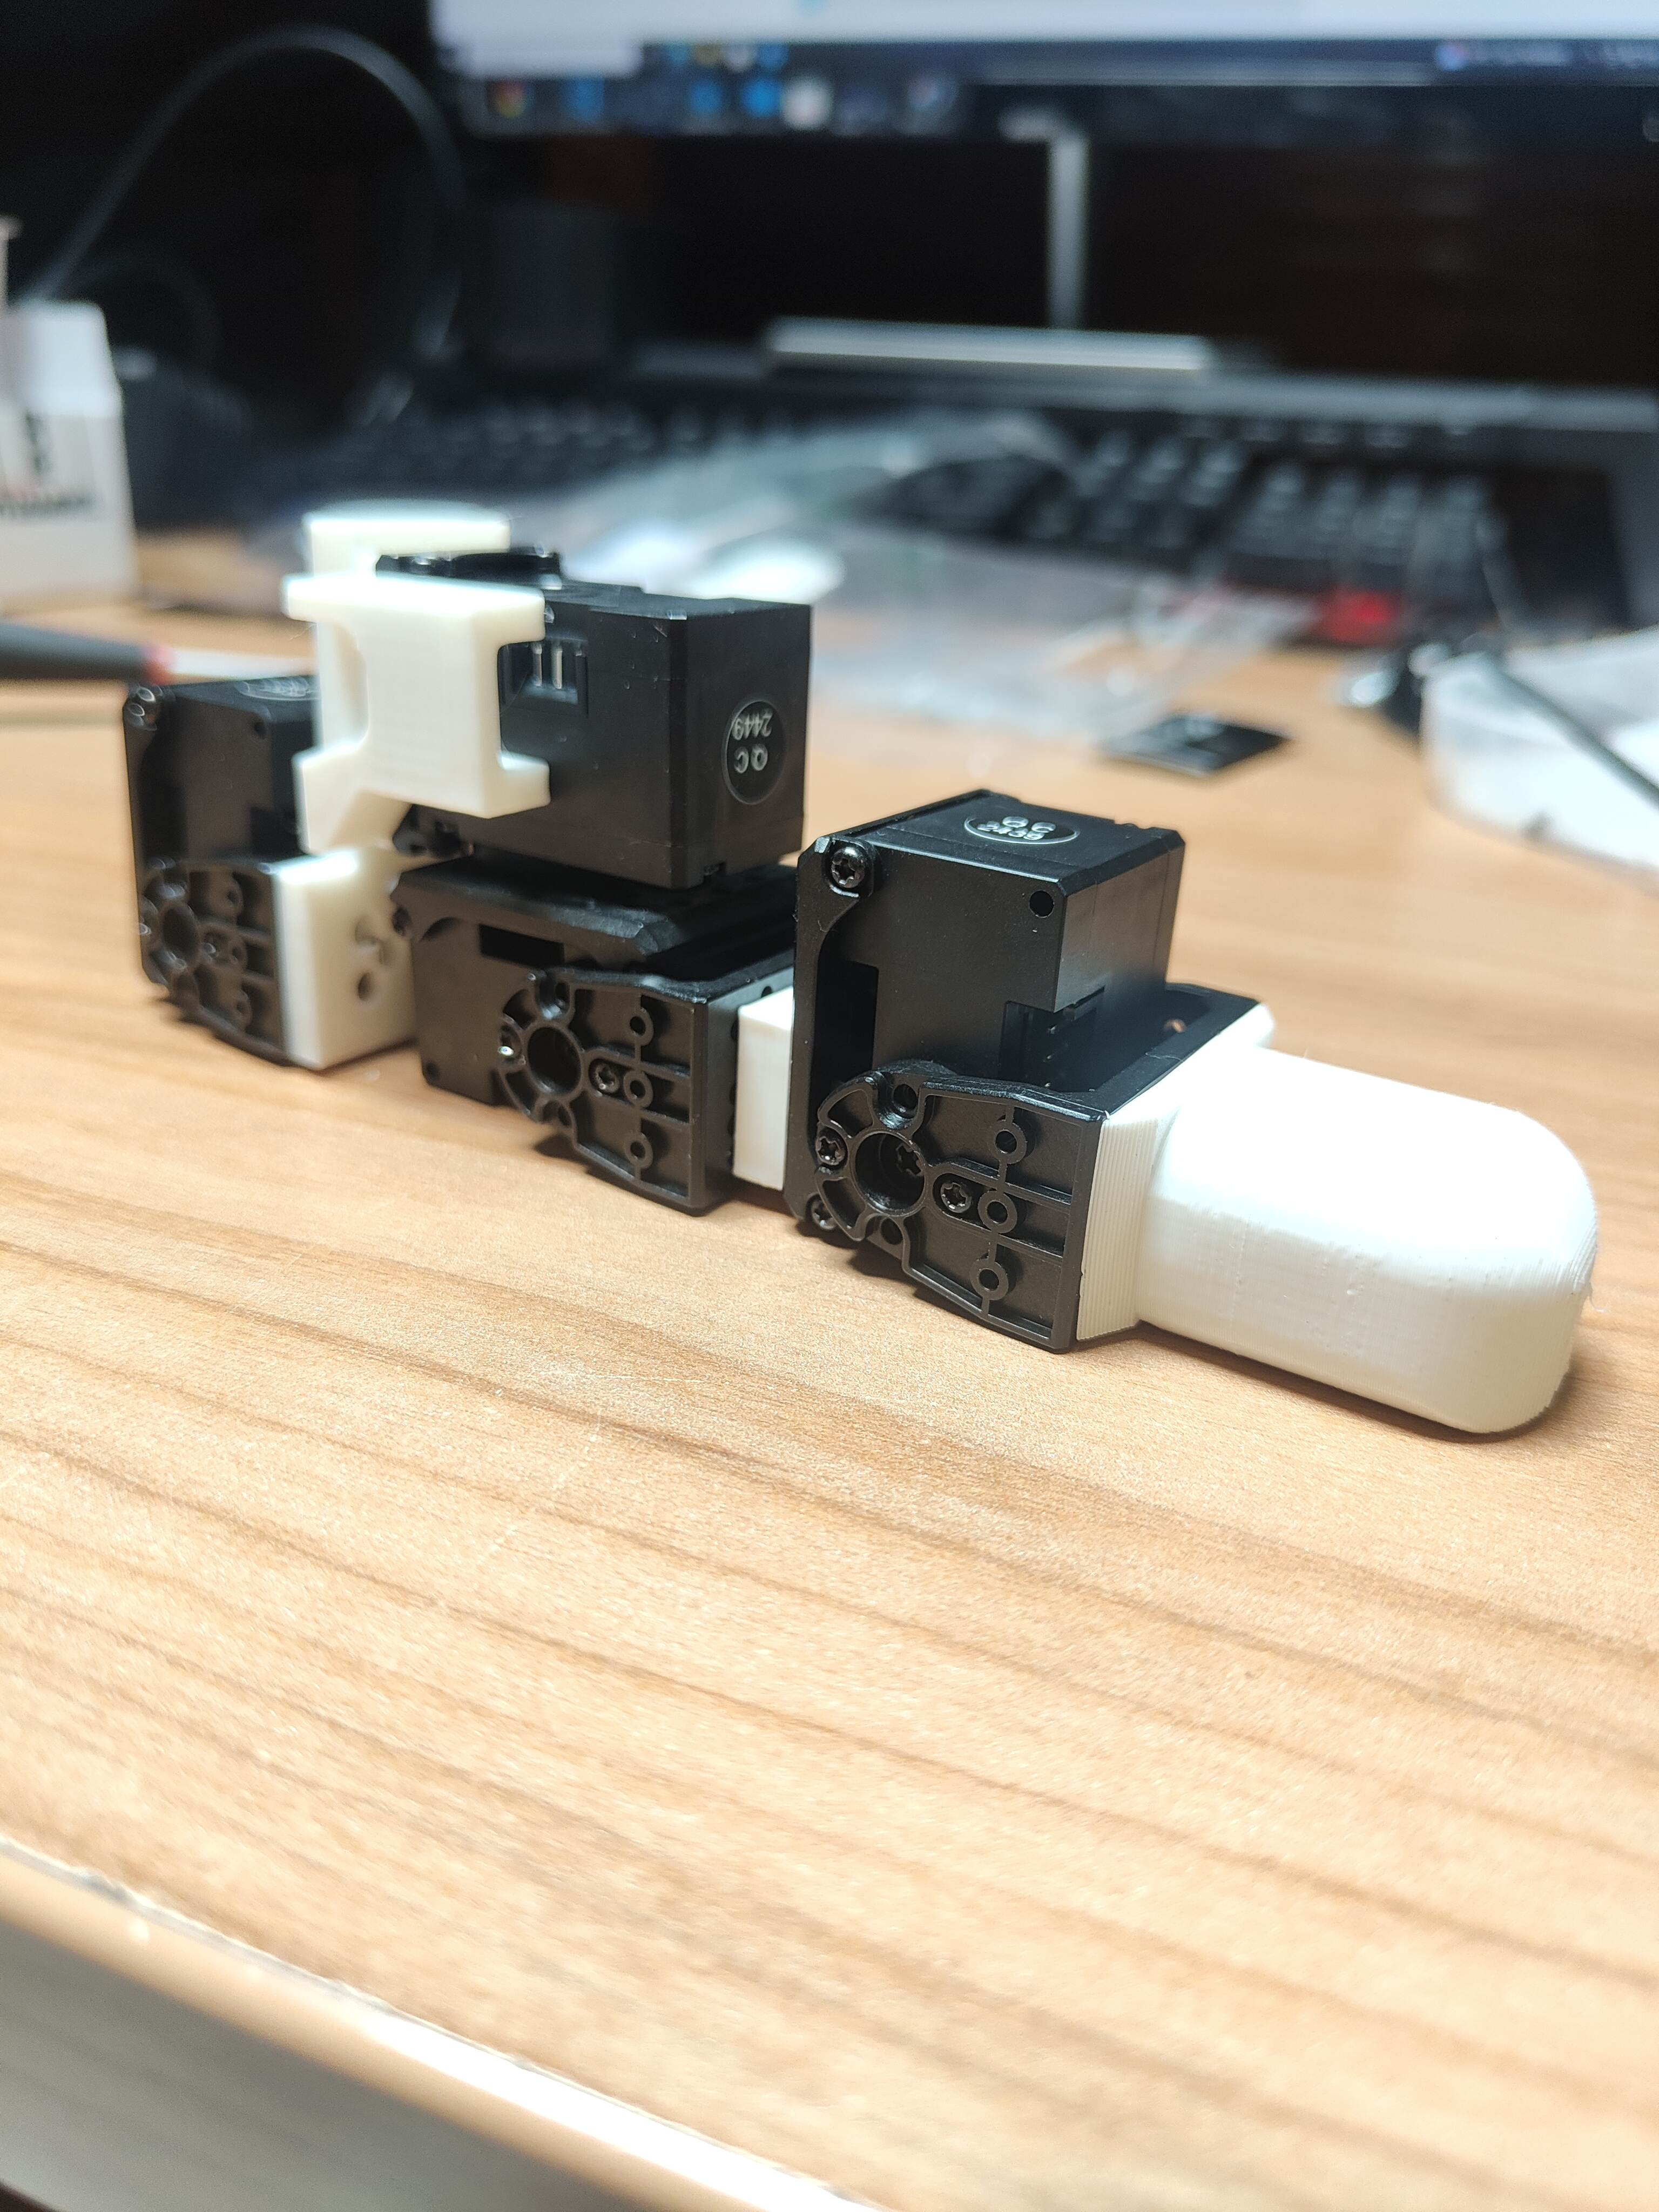
\includegraphics[height=6cm]{figs/chapter4/dedo.jpg}
        \caption{Dedo construído de acordo com a documentação da Leap Hand correspondente à estrutura do dedo indicador, médio e anelar}
        \label{fig:dedo}
    \end{minipage}
\end{figure}

No final do processo, obteve-se a mão totalmente montada, de acordo com a estrutura proposta na LEAP Hand, conforme ilustrado na Figura~\ref{fig:mao_montada}.

\begin{figure}[H]
    \centering
    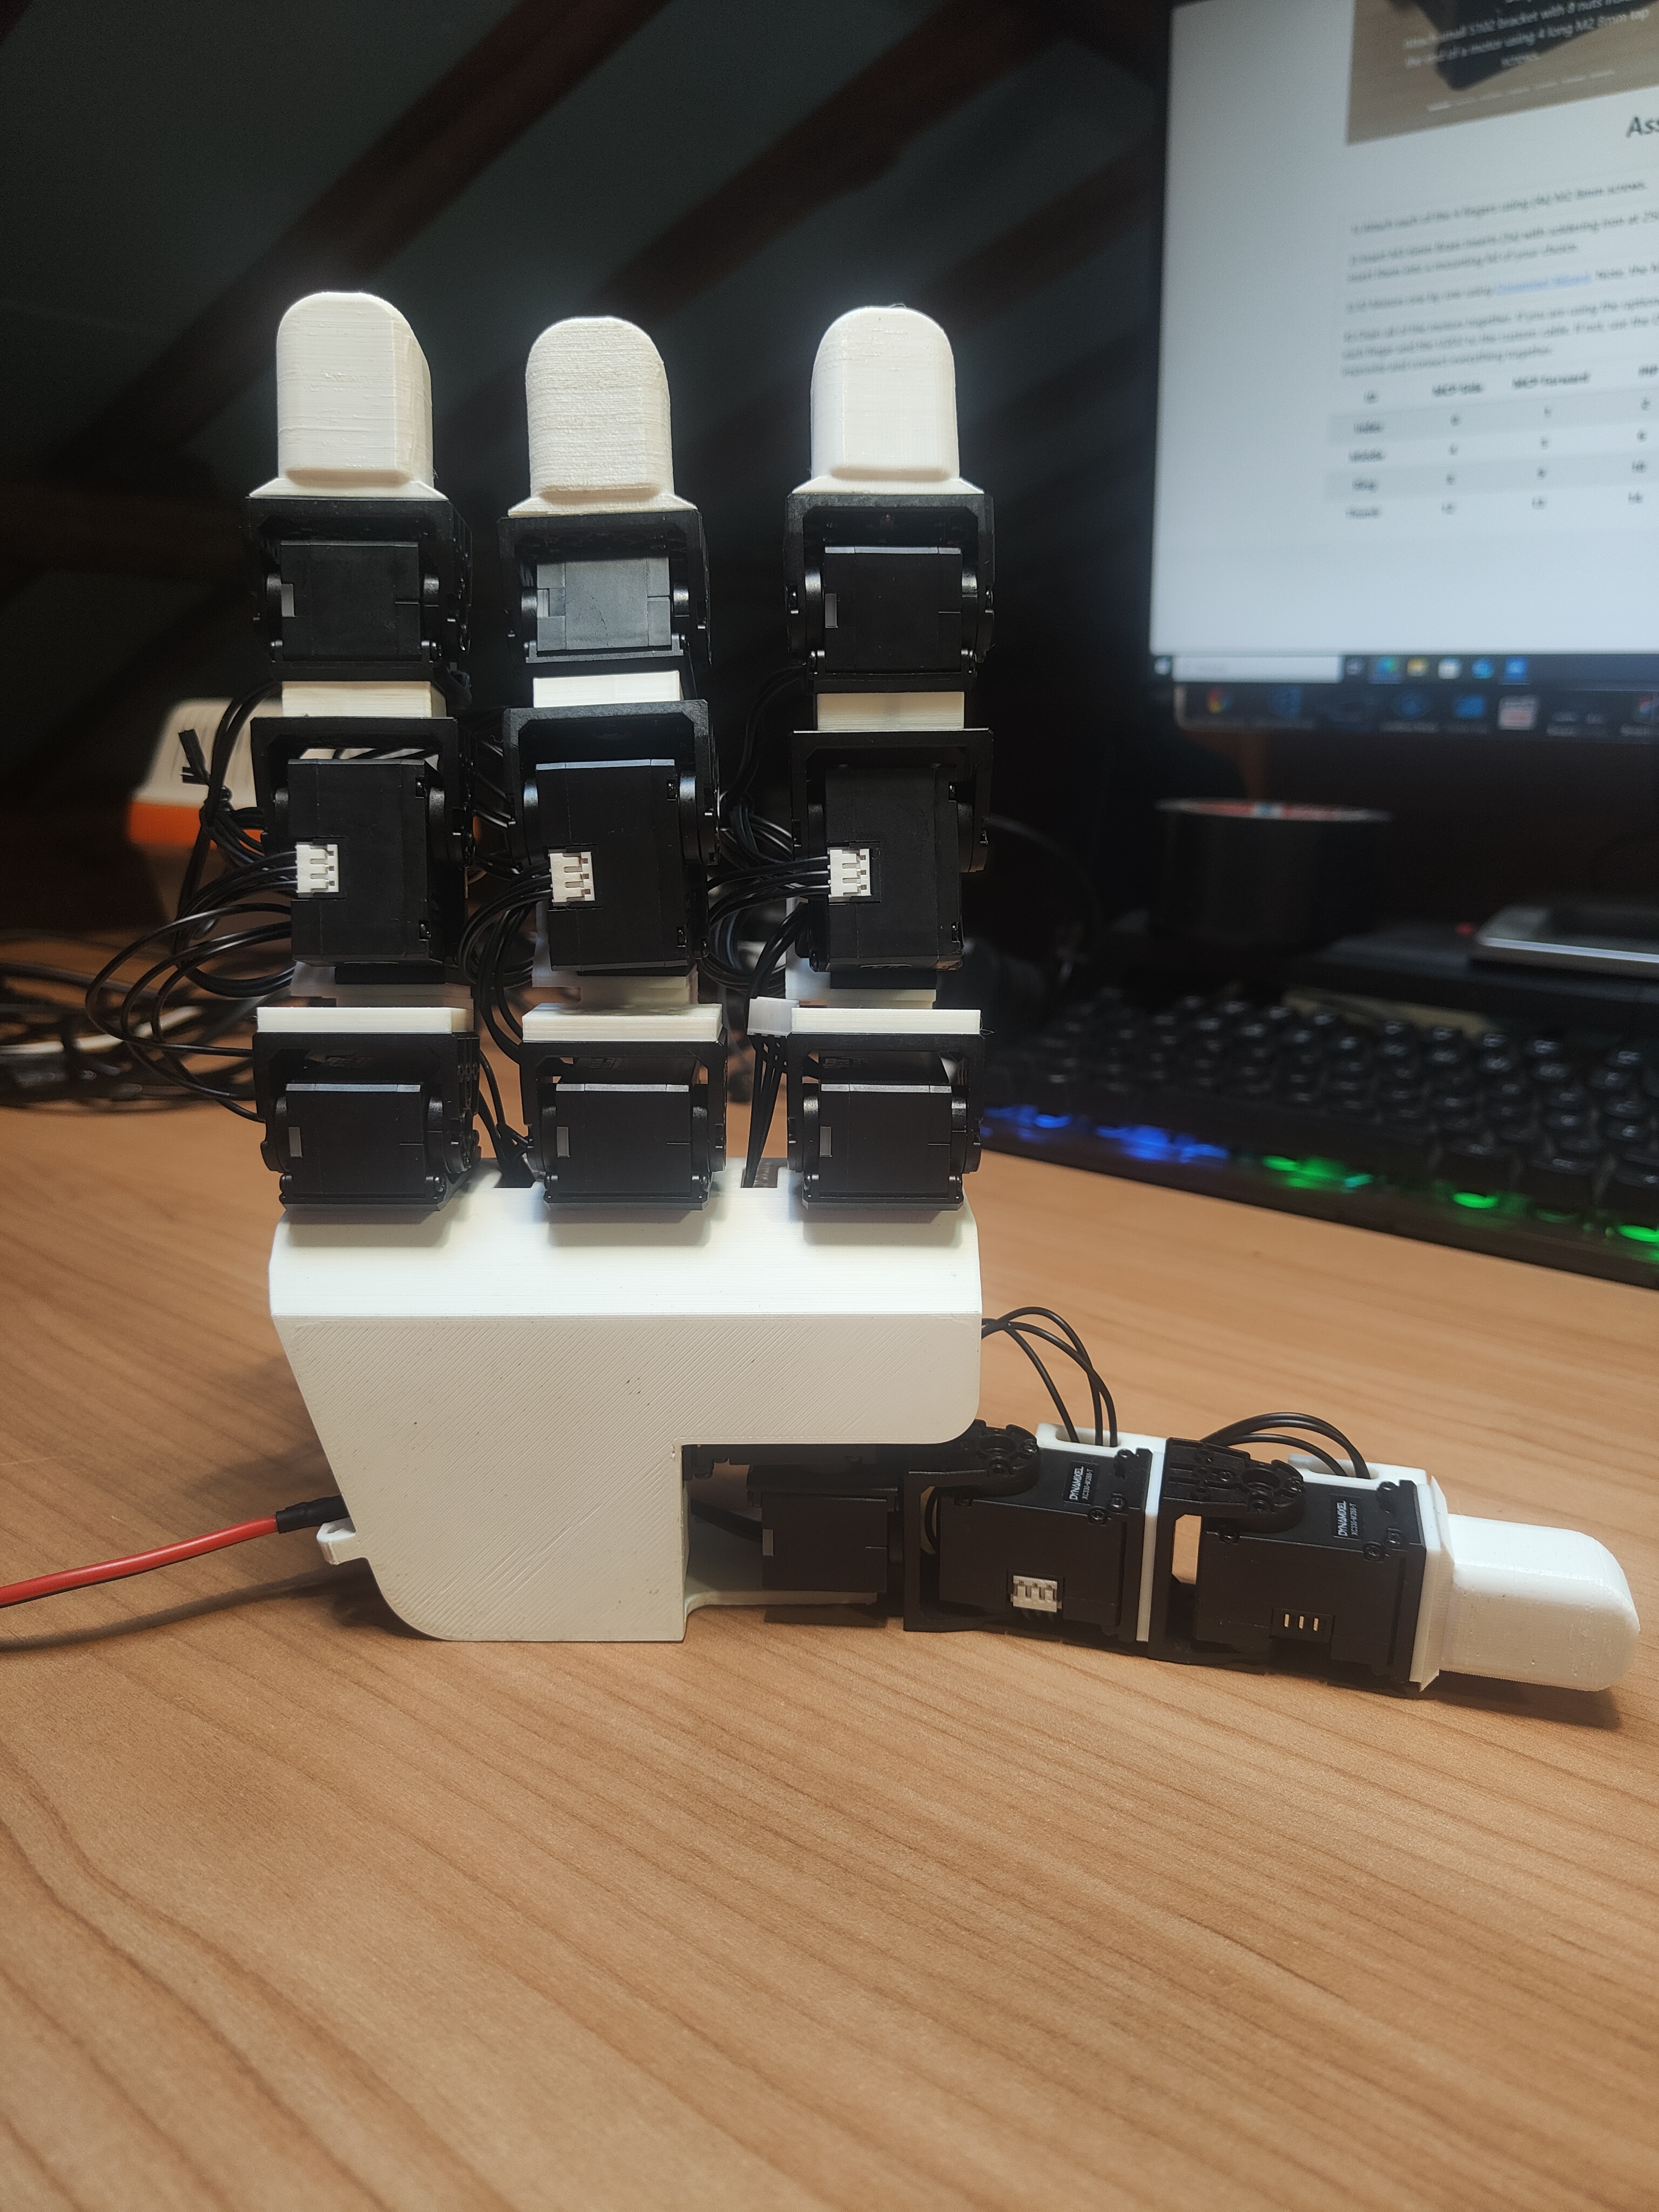
\includegraphics[height=8cm]{figs/chapter4/leap.jpg}
    \caption{Mão robótica completamente montada, seguindo a estrutura proposta na documentação da LEAP Hand.}
    \label{fig:mao_montada}
    
\end{figure}

Para complementar a descrição deste processo, no Apêndice~\ref{appendix:montagem_polegar} e ~\ref{appendix:montagem_dedo} e  são apresentadas imagens sequenciais representativas da construção de cada dedo, bem como hiperligações~\ref{appendix:videos} para vídeos que documentam o procedimento completo de montagem, constituindo assim um apoio visual adicional à documentação escrita.



Embora a montagem inicial tenha seguido rigorosamente as orientações da documentação da LEAP Hand, durante o desenvolvimento do projeto surgiram necessidades específicas que motivaram adaptações à estrutura original. Estas modificações serão detalhadas nas secções seguintes deste capítulo.



\subsection{Configuração dos Motores}

Antes de iniciar o desenvolvimento do código responsável pelo controlo dos movimentos da mão robótica, foi necessário proceder à configuração inicial dos motores Dynamixel. Esta fase incluiu a atribuição de identificadores únicos (IDs) a cada motor, uma vez que todos os motores, por defeito, vêm configurados com o mesmo ID. Para isso, recorreu-se à ferramenta gráfica Dynamixel Wizard 2.0, que permite, de forma intuitiva, alterar os parâmetros fundamentais de cada atuador.

Nesta configuração inicial, os IDs atribuídos seguiram a mesma lógica utilizada na documentação da LEAP Hand, garantindo assim compatibilidade com a estrutura de referência proposta pelos autores.

\subsubsection{Modos de Operação do Motores Dynamixel}

Após a atribuição dos IDs a cada motor, foi necessário configurar o modo de operação correspondente. Os motores Dynamixel XC330-M288-T suportam diversos modos de funcionamento, permitindo adaptá-los a diferentes tipos de movimentos e estratégias de controlo.

Na presente subsecção, são descritos os principais modos de operação disponibilizados por estes atuadores, destacando as suas características e o comportamento em situações com ou sem contacto com obstáculos.


\begin{enumerate}
    \item \textbf{Position Control Mode} \\
    Este modo permite definir uma posição angular específica que o motor deve atingir, dentro dos limites físicos configurados. Caso surja um obstáculo durante o movimento, o motor continuará a aplicar torque máximo na tentativa de alcançar a posição desejada, o que pode levar ao sobreaquecimento dos motores.


    \item \textbf{Extended Position Control Mode} \\
    Uma extensão do modo anterior, permite rotações superiores a 360°, tornando-se útil para aplicações que requerem movimento contínuo em rotação. No entanto, não é relevante no contexto deste projeto, dado que as juntas dos dedos não realizam rotações completas.


    \item \textbf{Velocity Control Mode} \\  
    Este modo permite definir uma velocidade angular constante, sem especificar uma posição final. O motor acelera até atingir a velocidade pretendida e mantém-se em rotação. Na presença de um obstáculo, o motor continua a tentar girar, aplicando o torque máximo, o que pode resultar em sobreaquecimento.


    \item \textbf{PWM Control Mode} \\
    Permite controlar diretamente a potência fornecida ao motor através de modulação por largura de pulso (PWM). Este modo oferece um controlo mais direto e flexível, mas não garante precisão de movimento, nem proteção contra obstáculos, podendo causar sobreaquecimento em situações de bloqueio mecânico.


    \item \textbf{Current Control Mode} \\
    Neste modo, controla-se diretamente o torque aplicado ao definir a corrente desejada. Se não houver resistência, o motor continua a girar. Na presença de um obstáculo, o motor não tenta forçar o movimento, e mantém um torque constante correspondente ao valor de corrente definido, oferecendo uma resposta segura e previsível.


    \item \textbf{Current-Based Position Control Mode} \\   
    Combina as vantagens do controlo de posição com limitação de corrente. O motor tenta alcançar uma determinada posição, mas limita o torque máximo aplicado, de acordo com o valor de corrente permitido. Se o obstáculo exigir mais torque do que o configurado, o motor interrompe o movimento, mantendo a força aplicada constante.

\end{enumerate}

A Tabela~\ref{tab:modos_operacao} resume os diferentes modos de operação, destacando os parâmetros controlados, as aplicações ideais e o comportamento em situações de contacto com obstáculos:

\begin{table}[H]
\centering
\begin{tabular}{l l p{6cm}}
\toprule
\textbf{Modo} & \textbf{Controla}  & \textbf{Reação a Obstáculos} \\
\midrule
Position Control & Posição & Aplica torque máximo até atingir posição \\
Extended Position & Posição ($>$360º) & Idêntico ao Position Control \\
Velocity Control & Velocidade  & Aplica torque máximo para manter velocidade \\
Current Control & Corrente (torque) & Mantém torque constante, sem tentar forçar \\
Current-Based Position & Posição + Corrente & Tenta atingir posição, mas respeita limite de torque \\
PWM Control & Potência (PWM) & Não protege contra sobrecarga ou obstáculos \\
\bottomrule
\end{tabular}
\caption{Resumo dos modos de operação dos motores Dynamixel}
\label{tab:modos_operacao}
\end{table}

A escolha do modo de operação adequado é essencial para garantir o desempenho desejado e a segurança do sistema. No contexto deste projeto, onde o contacto com objetos e a necessidade de limitar a força aplicada pelos dedos são aspetos fundamentais, foi escolhido o \textit{Current-Based Position Control Mode}, uma vez que este modo permite controlar a posição de cada articulação, ao mesmo tempo que impõe um limite ao torque aplicado, o que evita danos em situações de bloqueio ou contacto inesperado.


\subsection{Programação e Controlo}

A implementação do controlo dos motores Dynamixel exige, numa fase inicial, a correta definição dos parâmetros de comunicação, de forma a garantir a fiabilidade da ligação entre o sistema computacional e os atuadores.

Entre os elementos essenciais a configurar, destaca-se a especificação da porta serial utilizada, tipicamente \texttt{/dev/ttyUSB0} em sistemas operativos baseados em Linux, a taxa de transmissão de dados (\textit{baud rate}), o protocolo de comunicação (sendo utilizada a versão 2.0), a série dos motores (neste caso, a série X, correspondente aos modelos Dynamixel XC330-M288-T) e o identificador único (\textit{ID}) atribuído previamente a cada motor.

A correta parametrização destes elementos é fundamental para que seja possível estabelecer comunicação com os motores, enviar comandos de controlo e ler os parâmetros relevantes de operação. Nos pontos seguintes, descreve-se de forma progressiva a programação de um motor individual, o controlo coordenado de um dedo completo e, por fim, a implementação da lógica de controlo da mão robótica na sua totalidade.



\subsubsection{Programação de um motor individual}


A programação de um motor individual constitui o primeiro passo no desenvolvimento da lógica de controlo da mão robótica.
O processo tem início com a importação da biblioteca e a configuração da interface de comunicação serial. Tal configuração é efetuada através da criação dos objetos \texttt{portHandler} e \texttt{packetHandler}, com as instruções \texttt{portHandler = PortHandler(DEVICENAME)} e \texttt{packetHandler = PacketHandler(PROTOCOL\_VERSION)}. O primeiro estabelece a ligação física à porta serial especificada (por exemplo, \texttt{/dev/ttyUSB0}), enquanto o segundo gere a codificação e descodificação dos pacotes de dados, de acordo com o protocolo de comunicação adotado (neste projeto, a versão 2.0).


Após a abertura da porta e a verificação do sucesso da ligação, é necessário ativar o torque do motor para que este possa responder aos comandos enviados. A partir deste momento, torna-se possível controlar diversos parâmetros do motor, como a posição, a velocidade e a corrente máxima, dependendo do modo de operação previamente selecionado.

A leitura e escrita desses parâmetros nos registos internos do motor são realizadas através das funções disponibilizadas pelo SDK. A leitura pode abranger dados como a posição atual, velocidade de rotação, corrente consumida ou valor de PWM. A escolha da função adequada depende da dimensão dos dados a transferir, sendo comum o uso de \texttt{read2ByteTxRx()} e \texttt{read4ByteTxRx()} para valores de 2 e 4 bytes, respetivamente.

É importante salientar que os motores Dynamixel não fornecem diretamente a posição angular em graus ou radianos. Em vez disso, utilizam um sistema interno de representação baseado em \textit{ticks}, no qual a posição é expressa por um valor inteiro. No caso do modelo \texttt{XC330-M288-T}, a resolução do encoder é de 12 bits, o que resulta em $2^{12} = 4096$ valores distintos ao longo de uma rotação completa de $360^\circ$. Deste modo, cada unidade (\textit{tick}) corresponde a um incremento angular de aproximadamente $0{,}088^\circ$.

A conversão do valor lido, em \textit{ticks}, para a correspondente posição angular em graus é efetuada através da equação~\eqref{eq:conversao_graus}:

\begin{equation}
\theta = \frac{360 \times \text{ticks}}{4096}
\label{eq:conversao_graus}
\end{equation}

onde $\theta$ representa a posição angular em graus, e \texttt{ticks} é o valor devolvido diretamente pelo motor.

De forma análoga, a velocidade de rotação também é representada em \textit{ticks}. Neste caso, a relação com as unidades físicas é definida por um fator de conversão fornecido pelo fabricante. Para o motor em questão, cada unidade corresponde a aproximadamente 0{,}229 rotações por minuto (RPM). Assim, a velocidade real pode ser obtida através da equação~\eqref{eq:conversao_rpm}:

\begin{equation}
\text{Velocidade (RPM)} = \text{ticks} \times 0.229
\label{eq:conversao_rpm}
\end{equation}

Adicionalmente, o sinal do valor atribuído à velocidade determina o sentido de rotação: valores positivos indicam rotação no sentido horário, enquanto valores negativos correspondem a uma rotação no sentido anti-horário.

No que diz respeito à corrente elétrica consumida pelo motor, esta é diretamente disponibilizada pelo SDK em miliamperes (mA), não sendo necessária qualquer conversão adicional. Este parâmetro está diretamente relacionado com o torque aplicado pelo motor, sendo, por isso, relevante para o diagnóstico do esforço mecânico exigido durante o funcionamento.


\subsubsection{Programação e Controlo de um dedo}

Após a compreensão do funcionamento individual dos motores Dynamixel e da configuração dos seus parâmetros, procedeu-se ao desenvolvimento do controlo coordenado de um dedo completo da mão robótica. Cada dedo integra quatro motores, tornando necessário garantir a leitura sincronizada dos seus estados e o envio simultâneo de comandos de controlo, de forma eficiente e escalável.

Para tal, recorreu-se às funcionalidades de comunicação em bloco disponibilizadas pelo Dynamixel SDK, nomeadamente as operações \texttt{sync\_read}, \texttt{sync\_write}, \texttt{bulk\_read} e \texttt{bulk\_write}. No que respeita à leitura dos parâmetros dos motores — posição, velocidade e corrente — a função \texttt{sync\_read} foi a selecionada, por permitir aceder a um mesmo conjunto de registos em múltiplos motores de forma síncrona. Esta abordagem revelou-se eficiente tanto em termos de desempenho como de utilização de memória, além de respeitar as limitações de tamanho de mensagem impostas pelo protocolo de comunicação, evitando os riscos associados à utilização do \texttt{bulk\_read}.

Relativamente à escrita de comandos, optou-se pela função \texttt{bulk\_write}, que permite enviar dados distintos para registos diferentes de múltiplos motores numa única operação. Apesar de o registo alvo ser frequentemente o mesmo (como a posição ou o limite de corrente), esta escolha confere maior versatilidade ao sistema, permitindo a sua adaptação a cenários futuros em que diferentes parâmetros possam ser configurados seletivamente em cada motor.

Assim, a combinação de \texttt{sync\_read} para a leitura periódica do estado dos motores e \texttt{bulk\_write} para o envio de comandos de controlo assegura simultaneidade, escalabilidade e robustez no controlo coordenado de um dedo da mão robótica, servindo como base sólida para a extensão posterior ao controlo integrado de múltiplos dedos. Com esta abordagem, foi possível atingir uma taxa de leitura estável de aproximadamente 50Hz, garantindo uma monitorização suficientemente rápida para aplicações em tempo quase real.

Após implementar com sucesso o envio de comandos e a leitura simultânea dos parâmetros dos motores, procedeu-se à aplicação do modo de operação selecionado: o Current-Based Position Control Mode. A adaptação do código previamente desenvolvido foi direta, bastando configurar o registo correspondente ao modo de operação e definir um limite máximo de corrente na zona de inicialização do sistema. Esta configuração é realizada através da escrita nos endereços apropriados de cada motor Dynamixel.

Nos primeiros testes, foi definido um limite de corrente de 100mA. Embora este modo de operação não permita o controlo direto da velocidade, é possível estabelecer uma velocidade máxima por meio da configuração do parâmetro \texttt{Profile Velocity}. Assim, foram enviadas posições de destino previamente definidas para provocar o movimento de fecho e posterior abertura do dedo, com o objetivo de avaliar o comportamento dos motores em condições ideais. Os gráficos resultantes desta experiência encontram-se nas Figuras~\ref{fig:pos},~\ref{fig:vels} e ~\ref{fig:currs}.

\begin{figure}[H]
    \centering
    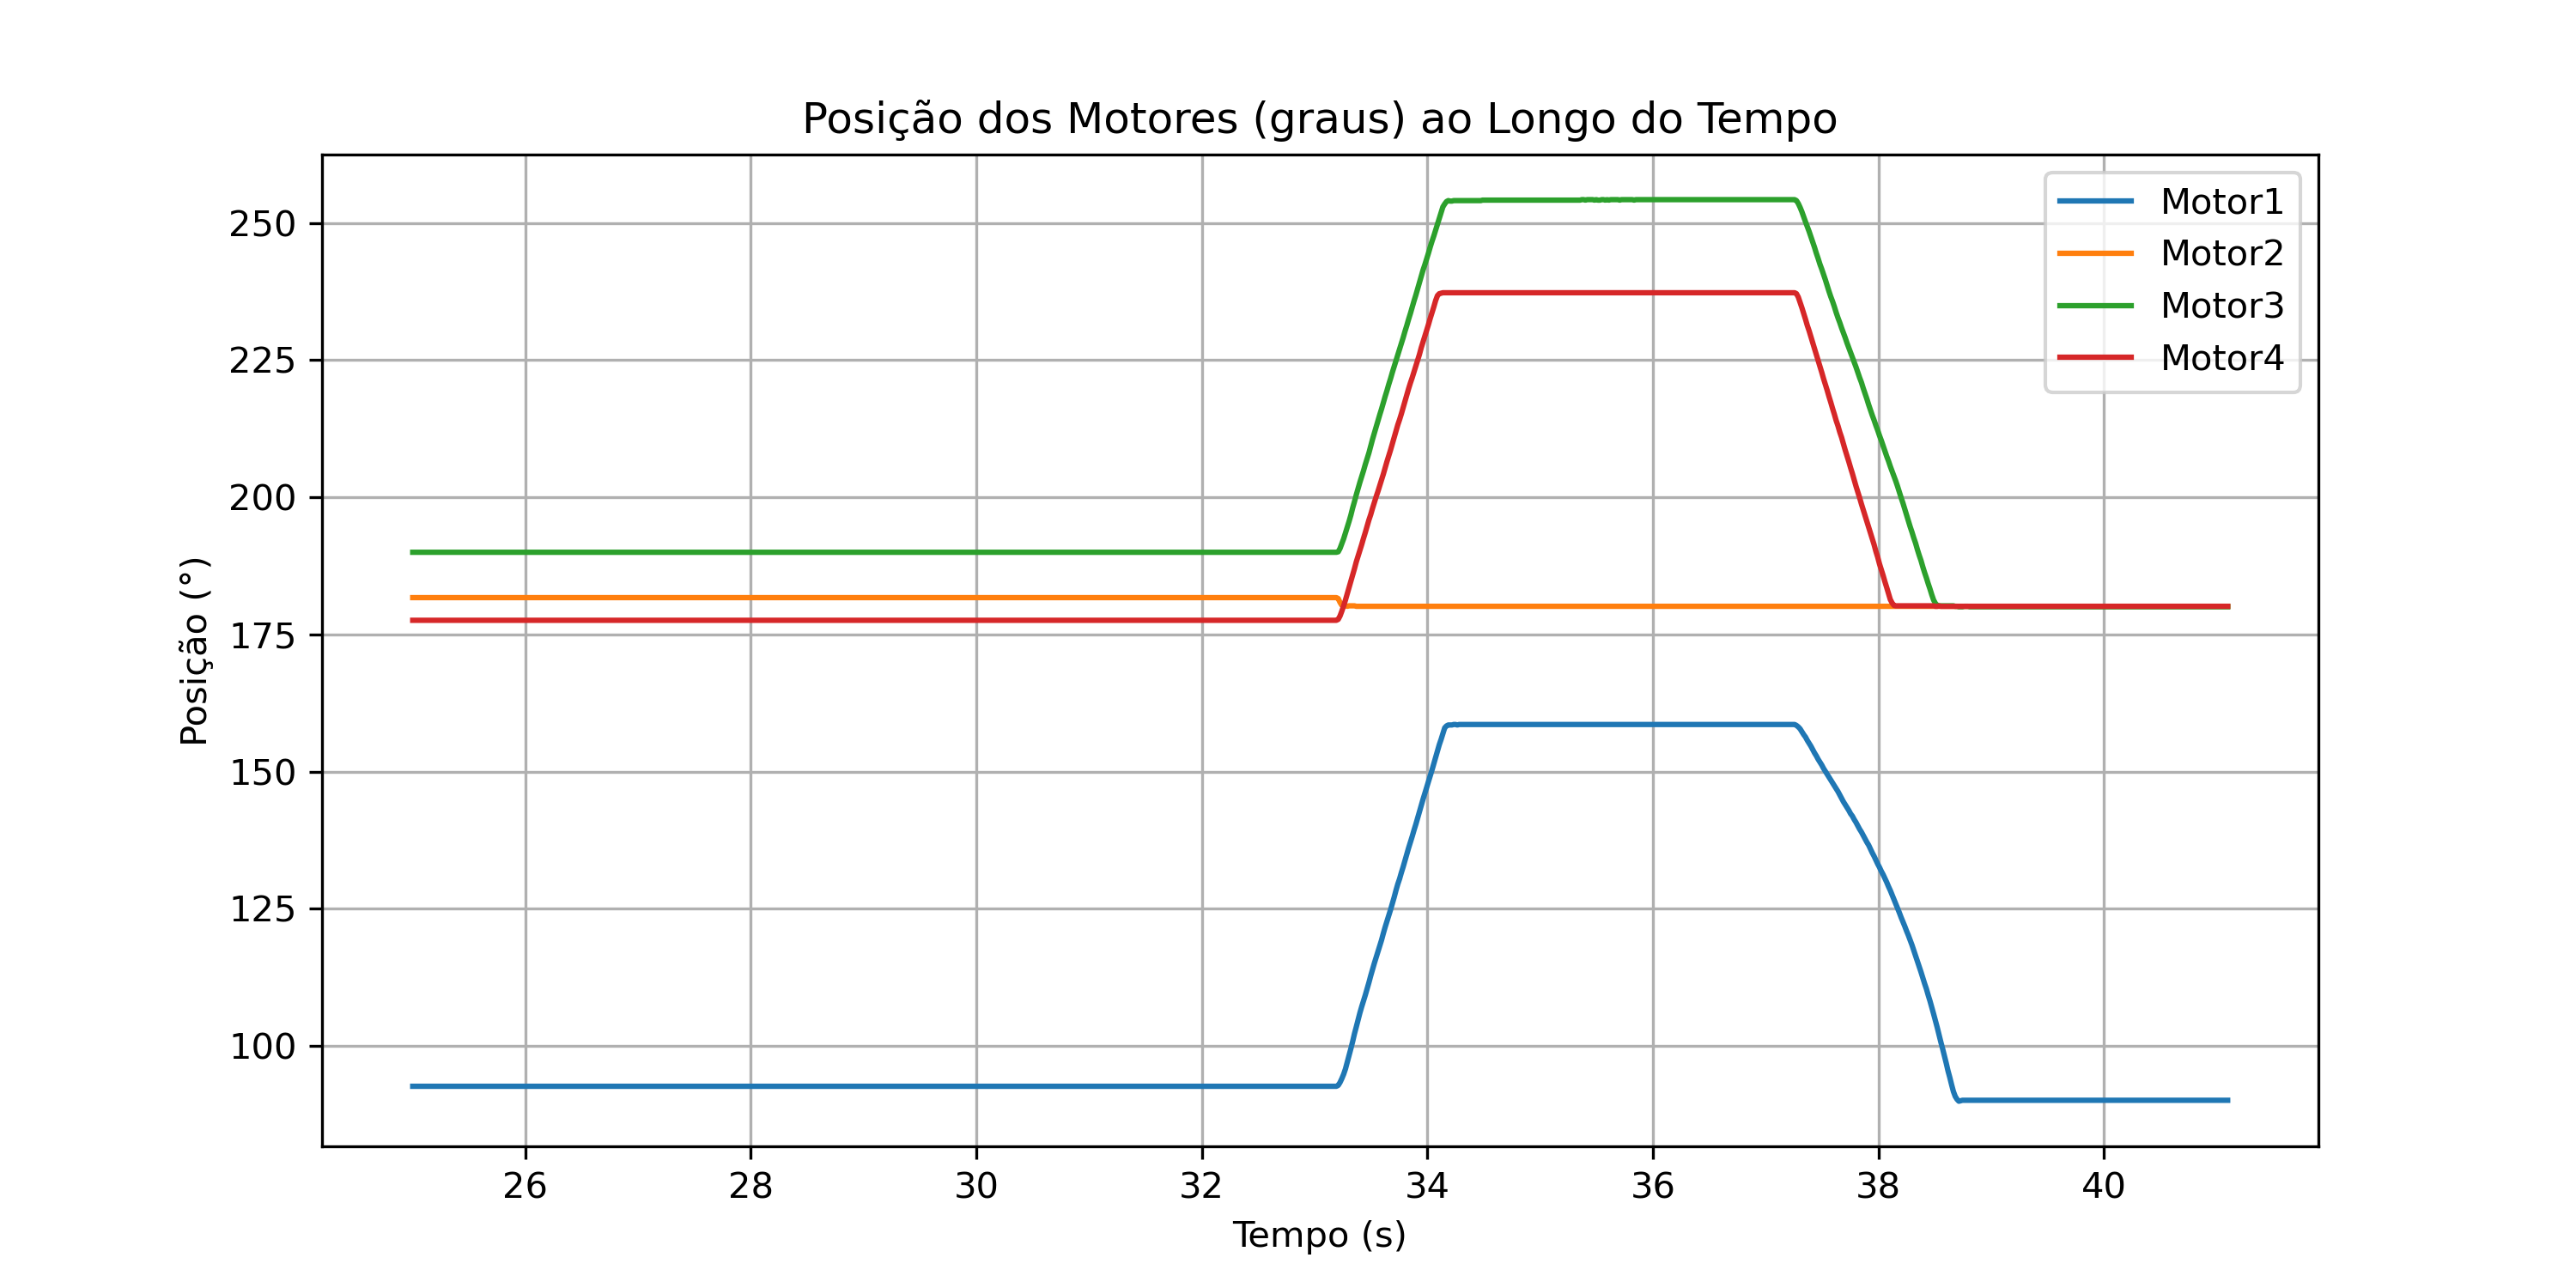
\includegraphics[height=6cm]{figs/chapter4/finger_positions.png}
    \caption{Posições dos motores ao longo do tempo durante o fecho e abertura do dedo sem nenhuma obstrução}
    \label{fig:pos}
    
\end{figure}
\begin{figure}[H]
    \centering
    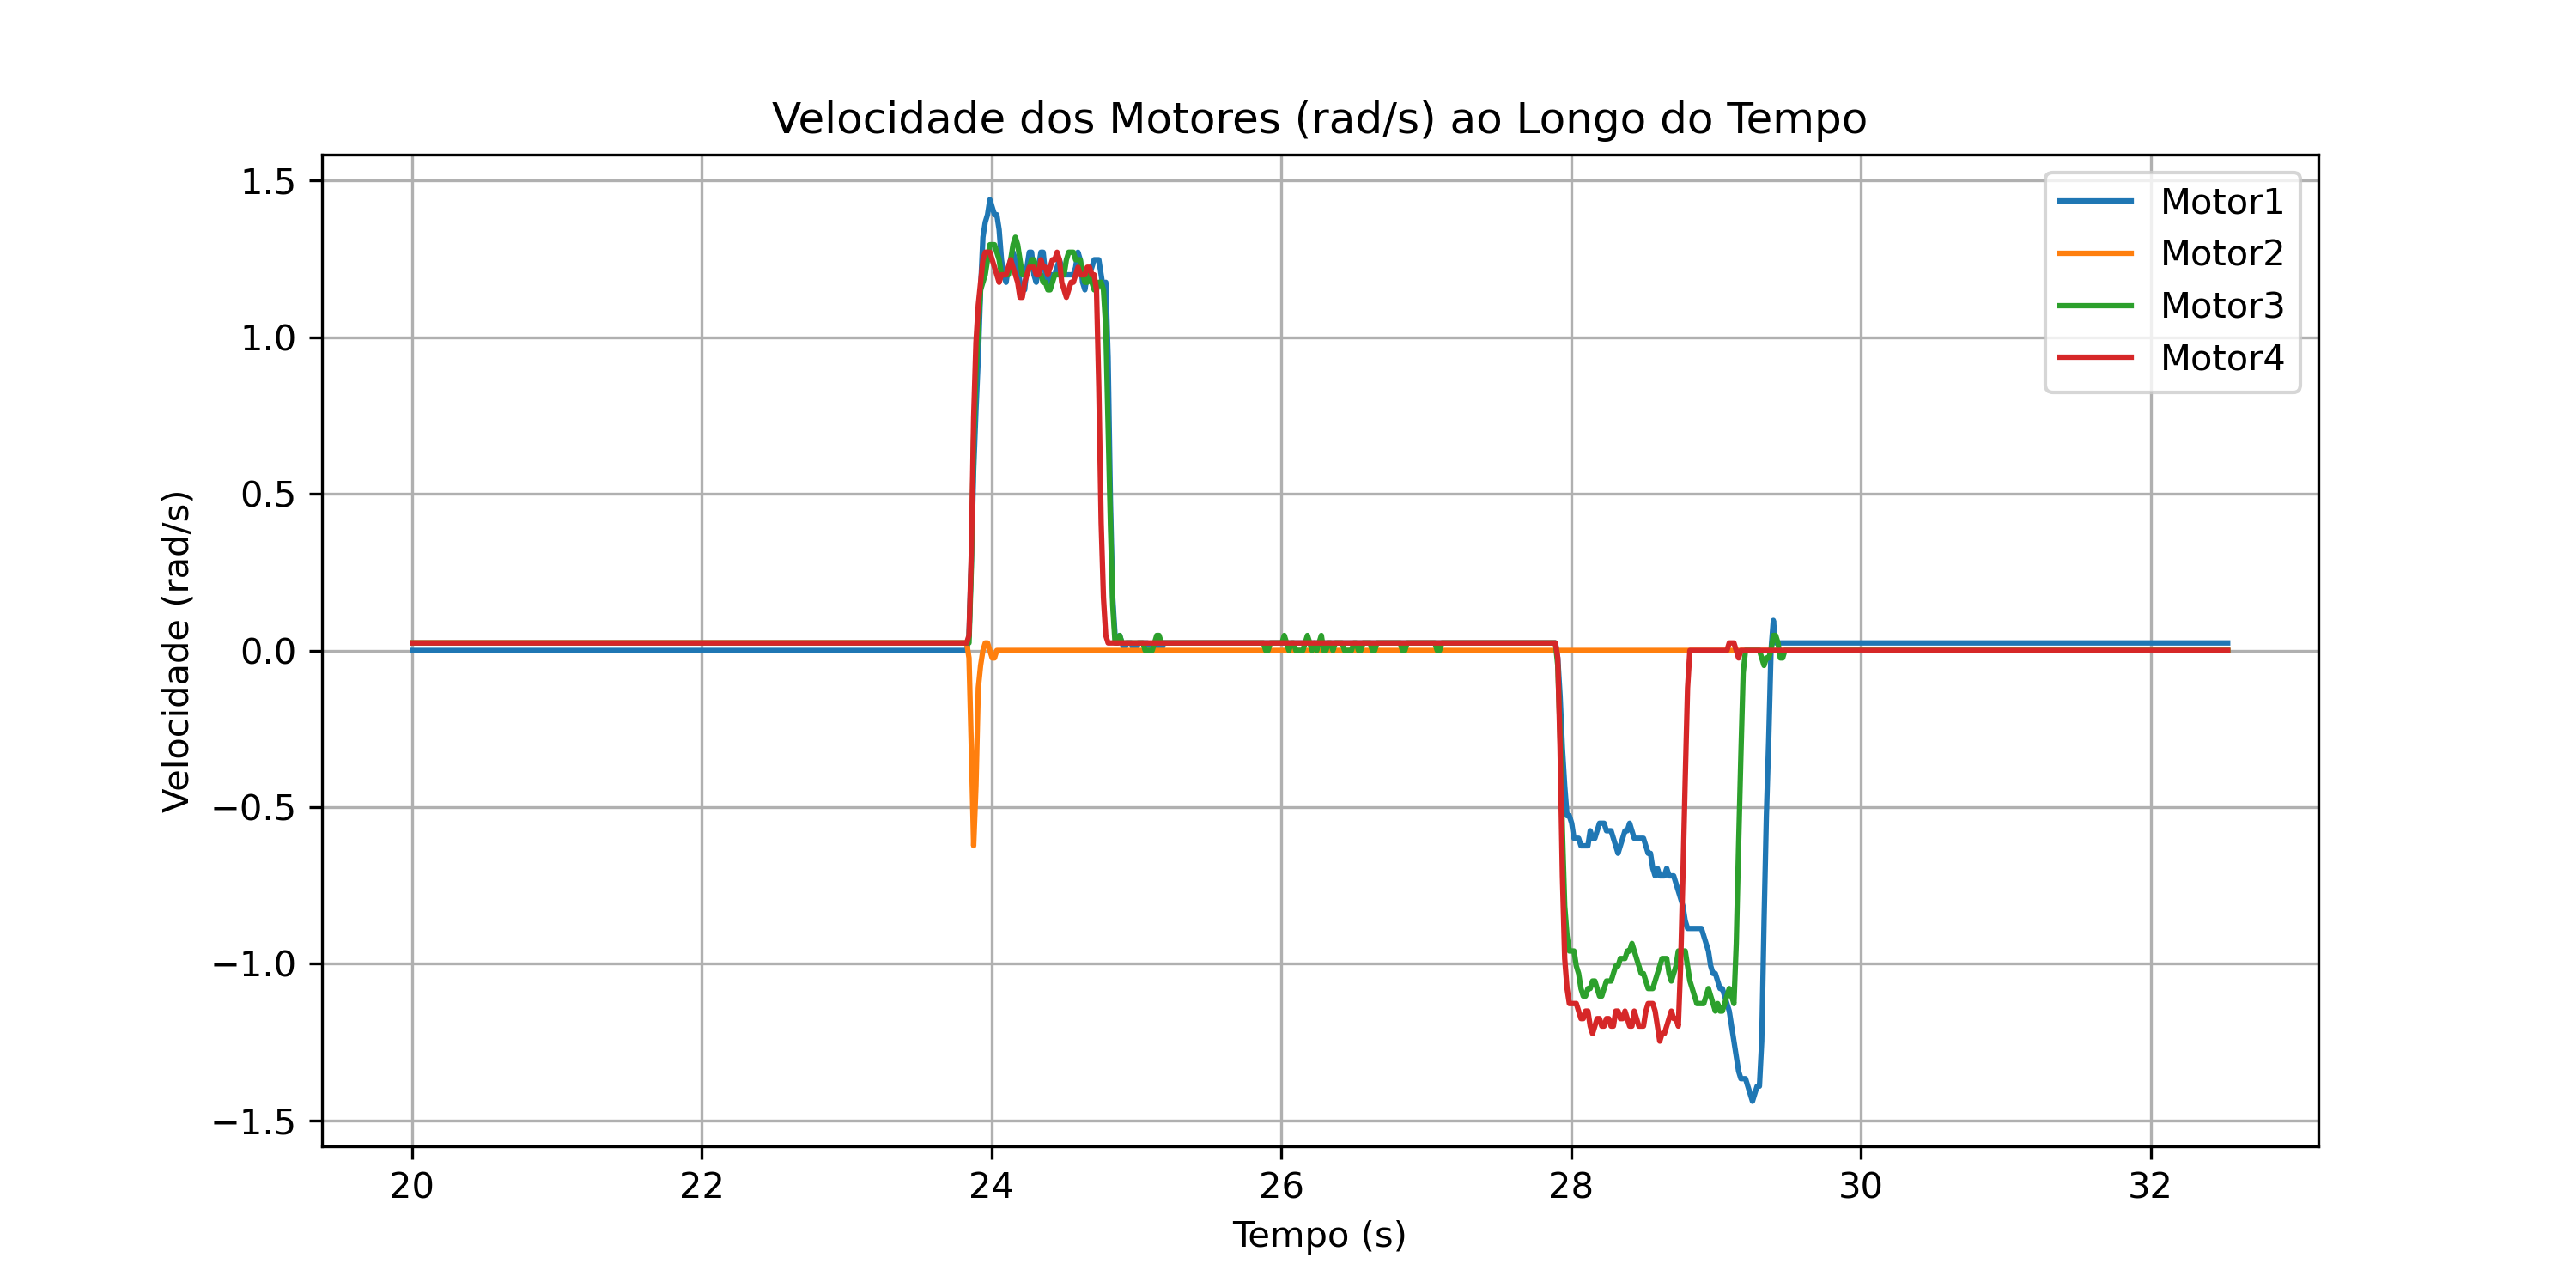
\includegraphics[height=6cm]{figs/chapter4/finger_velocities.png}
    \caption{Velocidades dos motores ao longo do tempo durante o fecho e abertura do dedo sem nenhuma obstrução}
    \label{fig:vels}
    
\end{figure}
\begin{figure}[H]
    \centering
    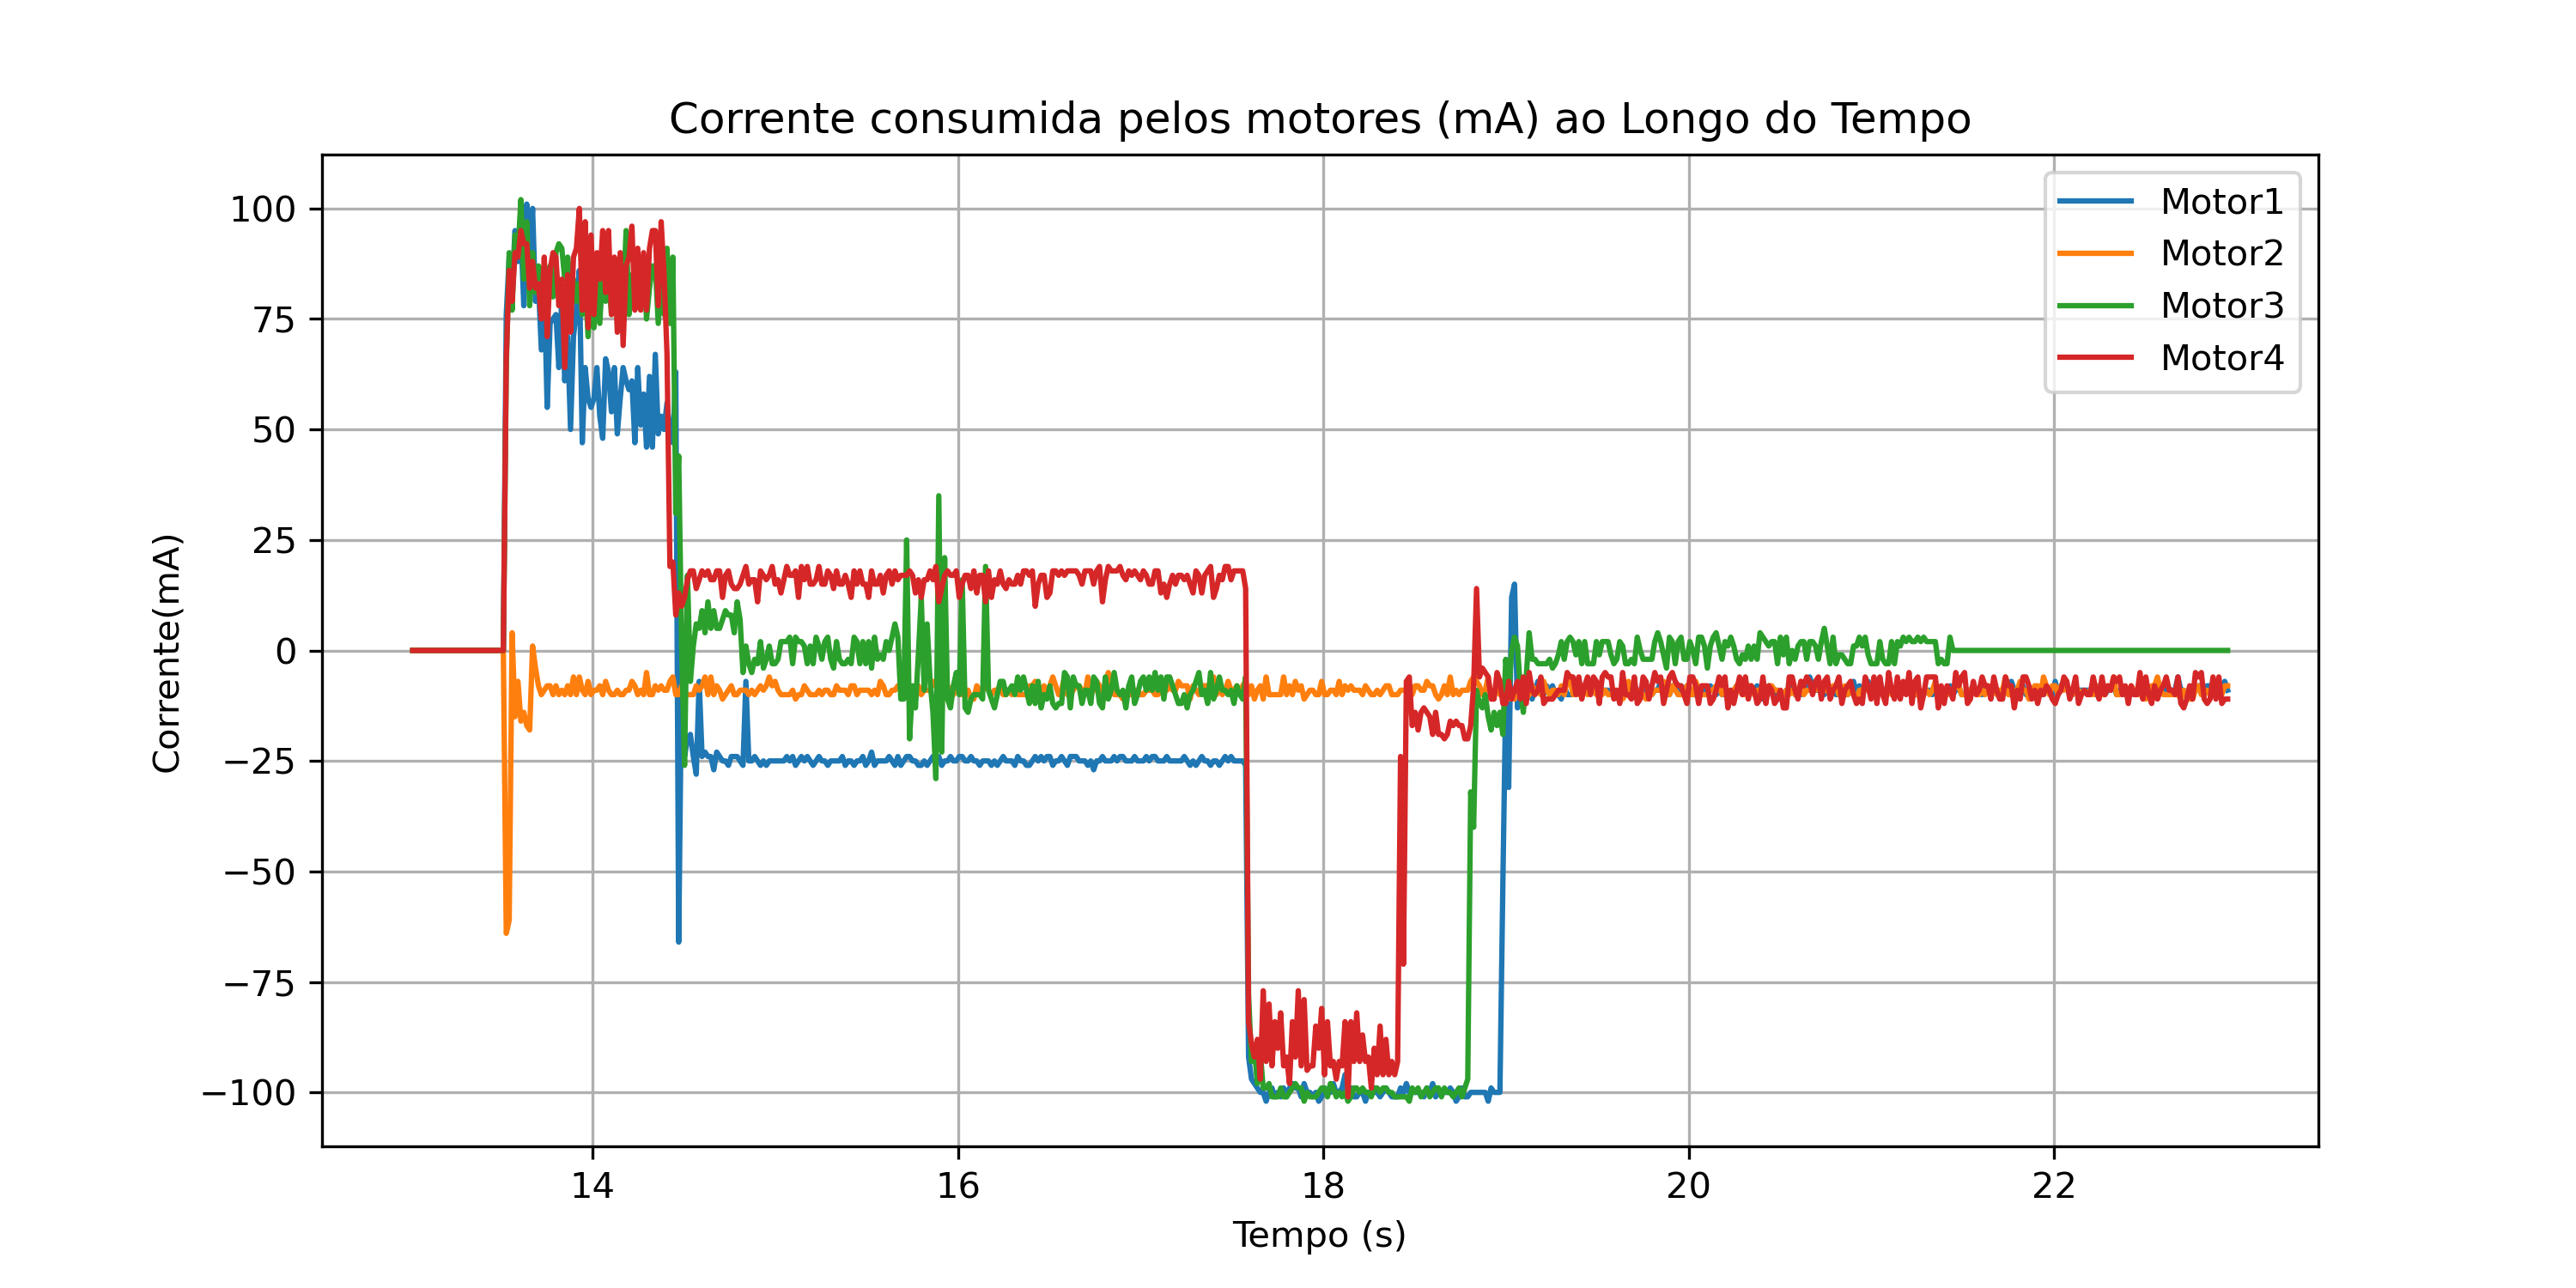
\includegraphics[height=6cm]{figs/chapter4/finger_currents.png}
    \caption{Correntes consumidas pelos motores ao longo do tempo durante o fecho e abertura do dedo sem nenhuma obstrução}
    \label{fig:currs}
    
\end{figure}

Como se pode observar, durante todo o movimento, os valores de corrente e velocidade mantiveram-se dentro dos limites especificados. A única exceção ocorreu no motor 1, onde se registou uma ligeira oscilação de velocidade, ultrapassando o valor definido em apenas 0.07 rad/s. Esta variação é considerada normal e esperada no funcionamento real dos motores, não comprometendo a estabilidade nem a segurança do sistema.

Na experiência seguinte, foram mantidas as mesmas posições de destino, mas introduziu-se um obstáculo físico que impedia a concretização do movimento pretendido. Tal como ilustrado nas Figuras~\ref{fig:pos1}, ~\ref{fig:vels1} e ~\ref{fig:currs1}, a análise dos dados revela diferenças claras entre os dois cenários. 

\begin{figure}[H]
    \centering
    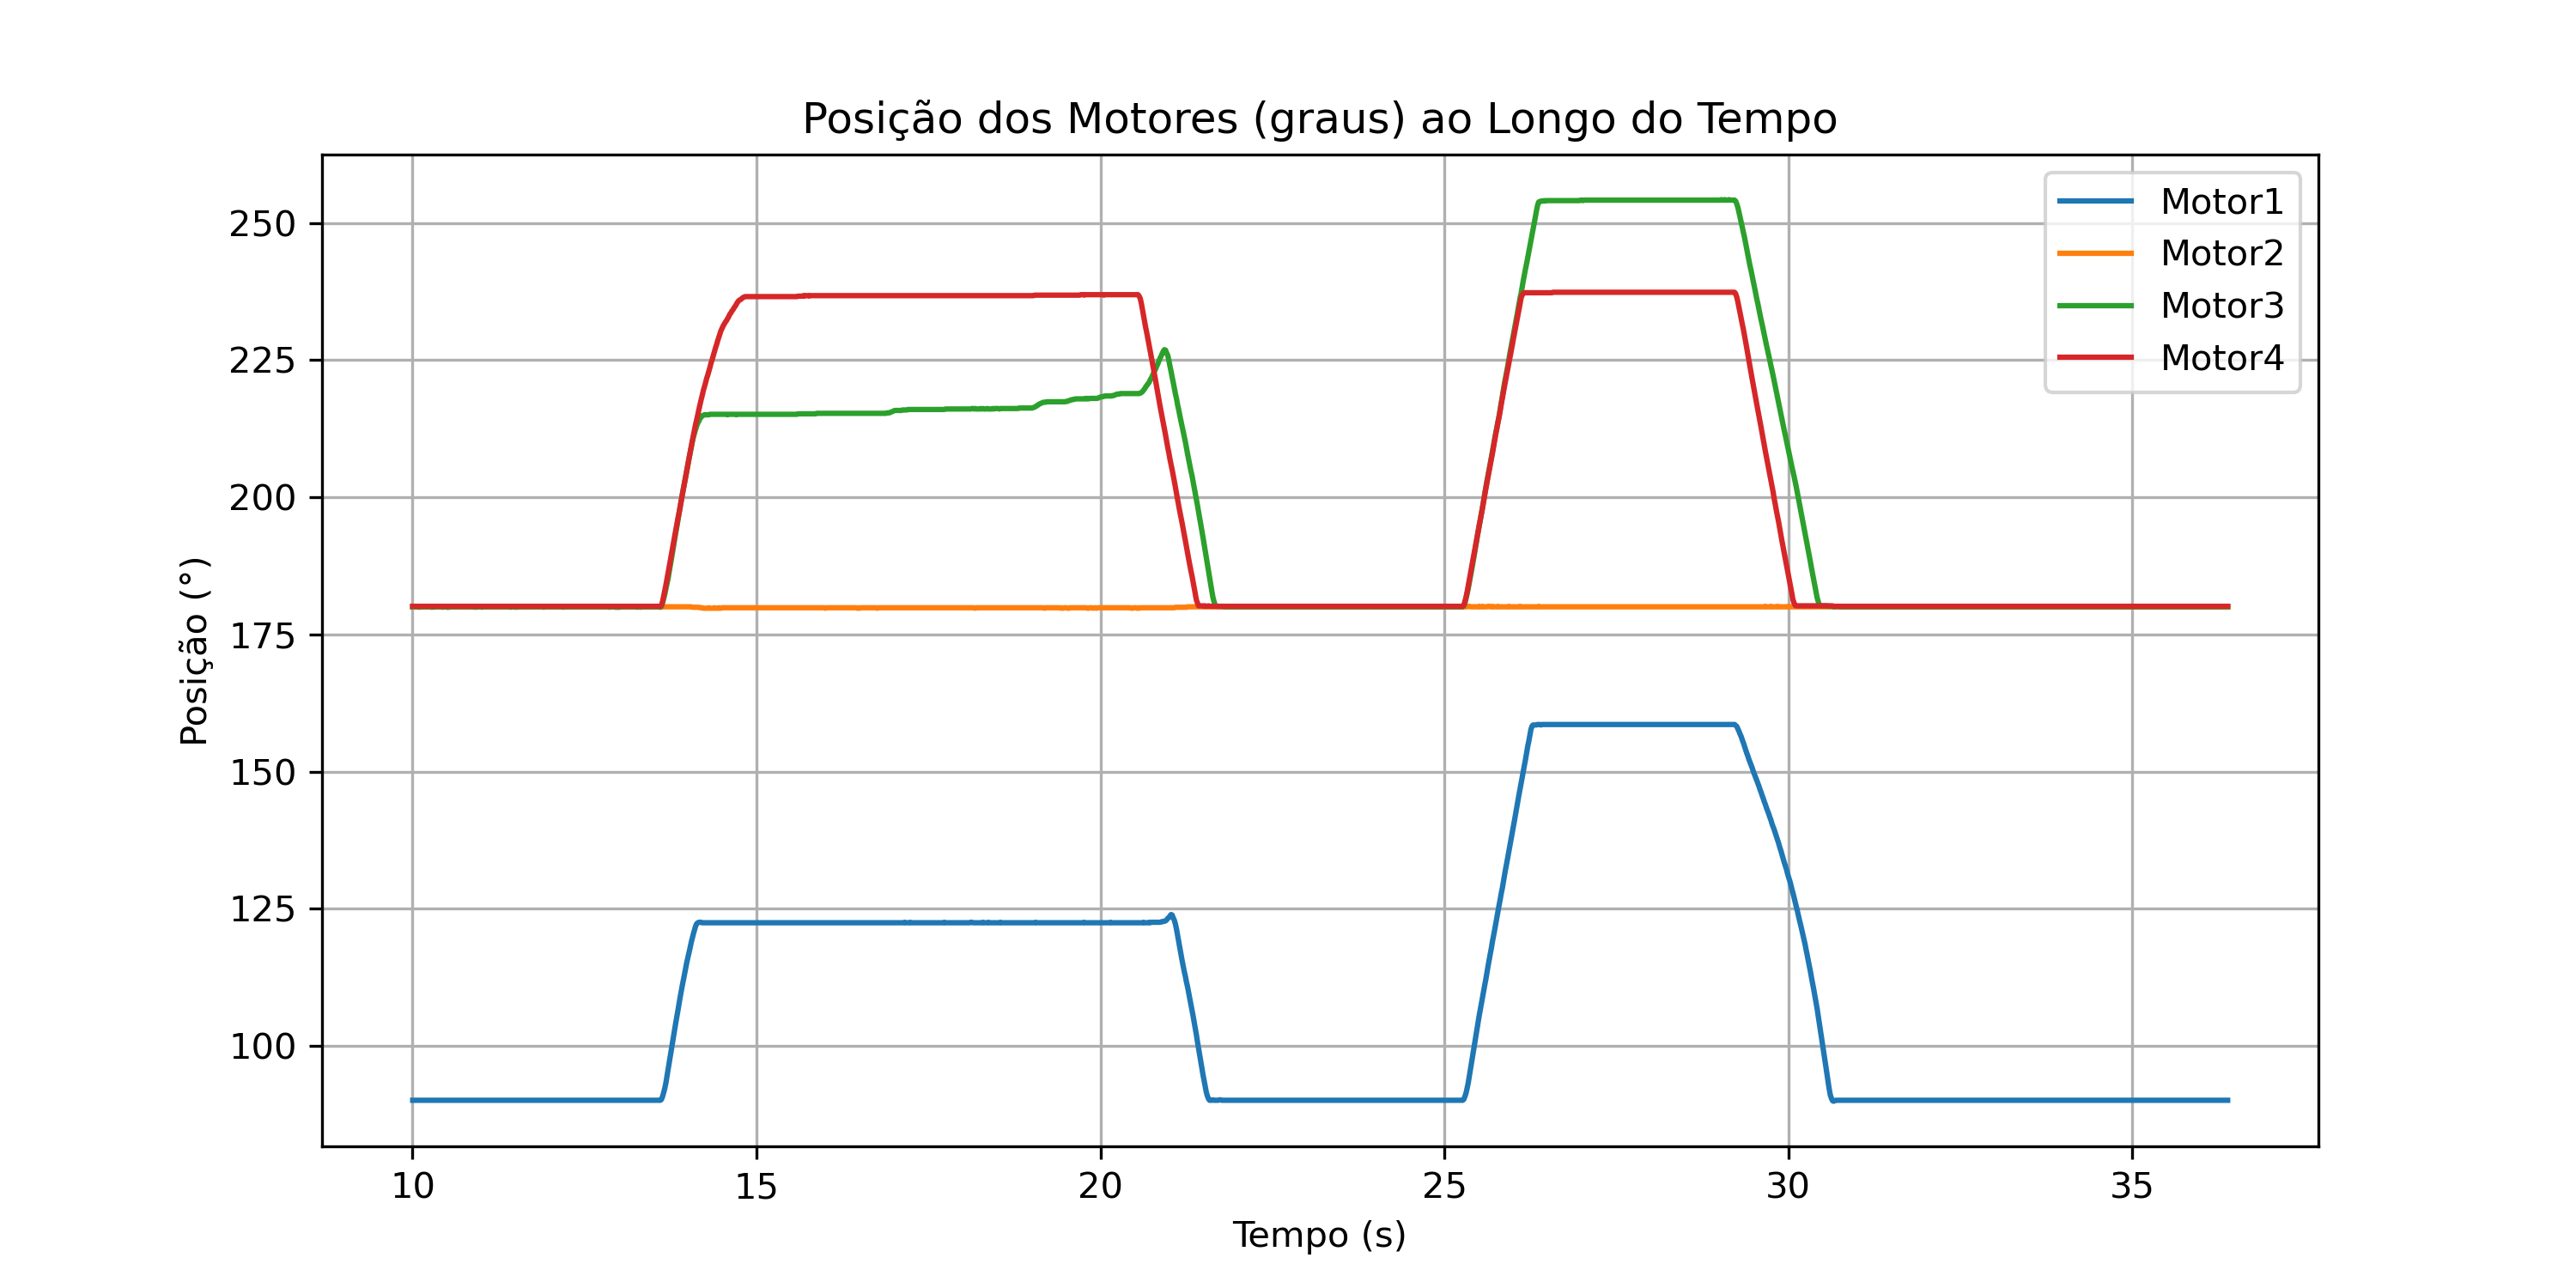
\includegraphics[height=6cm]{figs/chapter4/finger_positions_1.png}
    \caption{Posições dos motores ao longo do tempo durante o fecho e abertura do dedo com obstáculo}
    \label{fig:pos1}
    
\end{figure}
\begin{figure}[H]
    \centering
    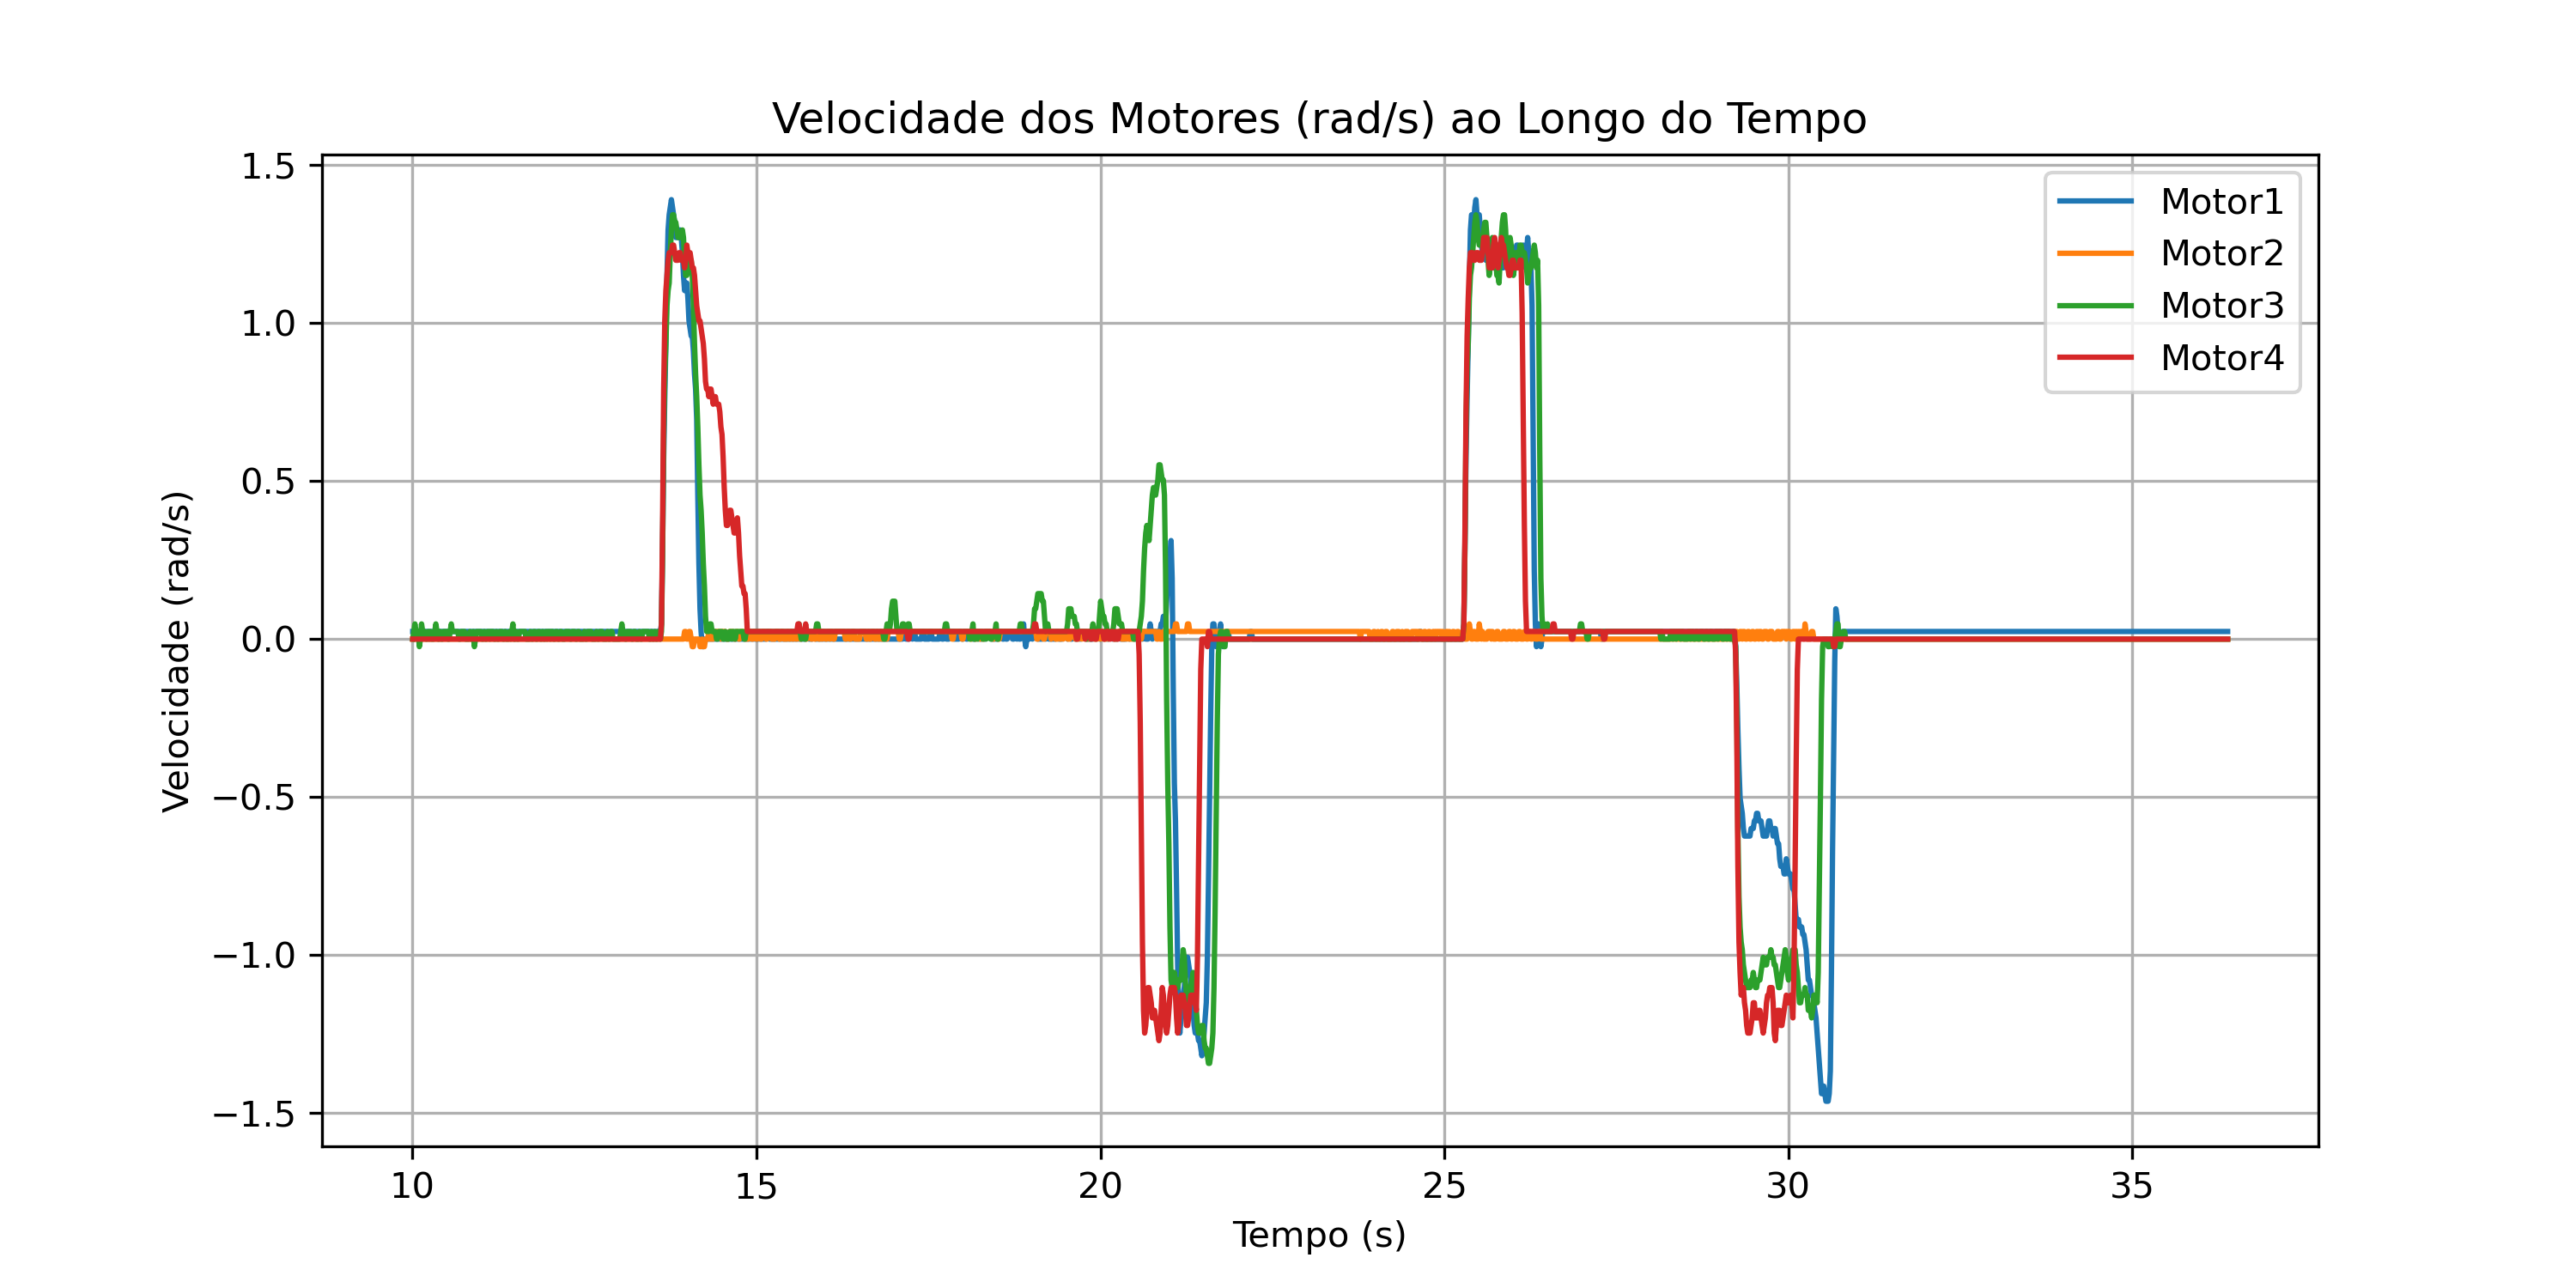
\includegraphics[height=6cm]{figs/chapter4/finger_velocities_1.png}
    \caption{Velocidades dos motores ao longo do tempo durante o fecho e abertura do dedo com obstáculo}
    \label{fig:vels1}
    
\end{figure}
\begin{figure}[H]
    \centering
    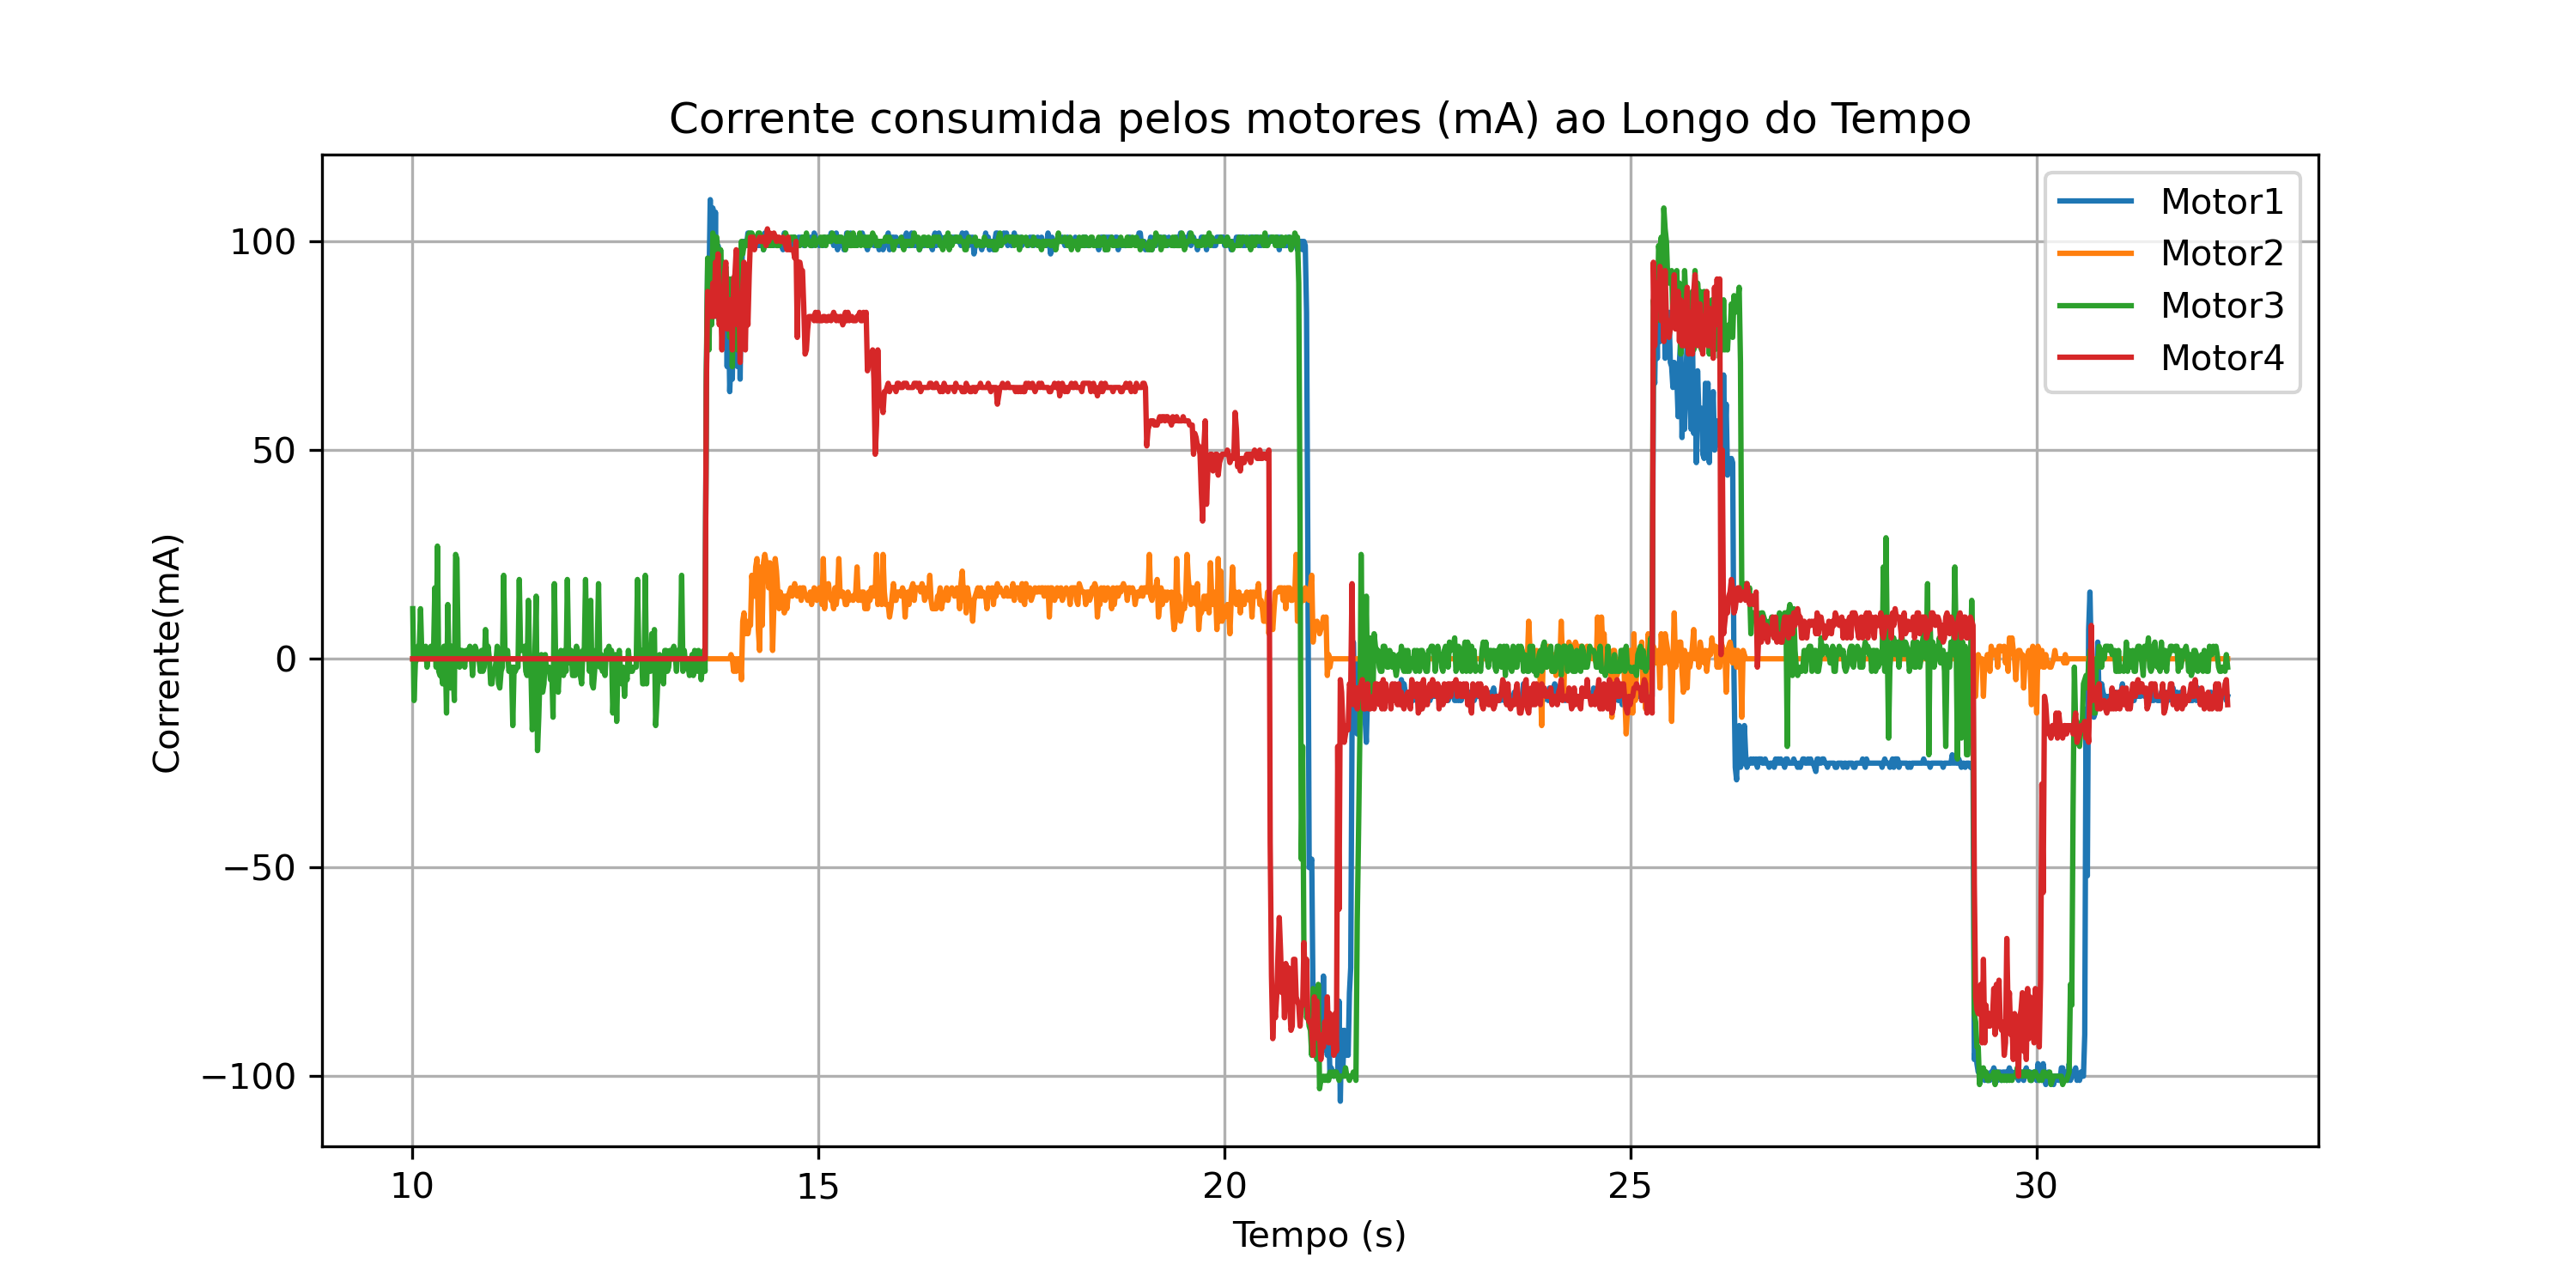
\includegraphics[height=6cm]{figs/chapter4/finger_currents_1.png}
    \caption{Correntes consumidas pelos motores ao longo do tempo durante o fecho e abertura do dedo com obstáculo}
    \label{fig:currs1}
    
\end{figure}

Na presença do obstáculo, o dedo não consegue atingir a posição alvo, resultando numa estabilização precoce da posição e no corte da velocidade. Simultaneamente, verifica-se um aumento significativo na corrente consumida, evidenciando o esforço do motor perante a resistência sem nunca ultrapassar o limite de corrente definido. Após a remoção do obstáculo, o sistema retoma o movimento normal, alcançando a posição desejada com maior estabilidade e menor consumo energético.

Estes resultados comprovam a utilidade e a eficácia do \textit{Current-Based Position Control Mode}, permitindo limitar a força exercida pelos motores durante a interação com o ambiente. Esta funcionalidade é fundamental para aplicações em que a segurança e a adaptabilidade ao contacto com objetos são essenciais, como é o caso da manipulação robótica.

Para além das duas experiências iniciais, foram conduzidos testes adicionais com o objetivo de aprofundar a análise do comportamento dos motores em diferentes condições operacionais. Numa dessas experiências, o dedo foi submetido a movimentos de abertura e fecho com diferentes velocidades máximas configuradas. Os resultados, apresentados no Apêndice~\ref{appendix:teste_velocidades}, demonstram que velocidades mais reduzidas conduzem a um menor consumo energético e a uma variação mais suave da posição ao longo do tempo. A inclinação menos acentuada da curva de posição indica um movimento mais progressivo e controlado, confirmando a influência direta da velocidade sobre a dinâmica do sistema.

Outra experiência relevante consistiu em introduzir obstáculos que interrompessem o movimento do dedo em diferentes posições, com o intuito de estudar o efeito da localização do obstáculo no comportamento individual dos motores. Verificou-se que, quando o obstáculo atua sobre a base do dedo (afetando os motores inferiores), apenas o motor bloqueado entra em esforço, enquanto os restantes continuam a tentar atingir as suas posições alvo. Em contraste, quando o obstáculo é colocado na extremidade do dedo, todos os motores são simultaneamente afetados, ficando em esforço e impedidos de completar o movimento. Esta experiência, cujos gráficos se encontram no Apêndice~\ref{appendix:teste_posições_obstaculos}, reforça ainda a eficácia do controlo baseado em corrente, uma vez que a corrente consumida em nenhuma circunstância ultrapassou o limite máximo previamente definido.

Os dados experimentais obtidos encontram-se acompanhados de gráficos e ligações para vídeos demonstrativos no Apêndice~\ref{appendix:teste_velocidades} e ~\ref{appendix:teste_posições_obstaculos}, permitindo uma análise visual clara dos diferentes comportamentos observados. Estas experiências complementares contribuem significativamente para a validação do sistema de controlo implementado, demonstrando não só a sua eficácia em cenários ideais, mas também a sua robustez perante interações físicas imprevistas.







\subsubsection{Programação da Mão completa}



\subsection{Arquitetura de Software Desenvolvida}



\subsection{Funcionalidades Avançadas}

\subsubsection{Ajuste dinâmico de corrente no contacto com objetos}

\subsubsection{Implementação de velocidades relativas entre dedos e falanges}

\subsubsection{Implementação de atrasos temporais programáveis entre movimentos de dedos}




\section{Implementação dos Sensores de Contacto}


\subsection{Seleção do Microcontrolador}







\subsection{Implementação Física do Sistema sensorial}

\subsubsection{Unidade de Aquisição dos sensores}

\subsubsection{Desenho da peça para fixação}

\subsubsection{Desenvolvimento do PCB}


\subsection{Testes com sensores}

\subsubsection{Testes iniciais com sensores FSR}

\subsubsection{Teste com sensor FSR 406}

\subsubsection{Desenho de Peça para propagar a força para o sensor}


\section{Conclusão}
